\documentclass{article}

% if you need to pass options to natbib, use, e.g.:
%     \PassOptionsToPackage{numbers, compress}{natbib}
% before loading neurips_2019

% ready for submission
\usepackage[nonatbib]{neurips_2019}
% \usepackage{neurips_2019}
% \usepackage[nonatbib,preprint]{neurips_2019}
% \usepackage[nonatbib,final]{neurips_2019}

\newcommand{\dds}{DDS}

\usepackage[utf8]{inputenc} % allow utf-8 input
\usepackage[T1]{fontenc}    % use 8-bit T1 fonts
\usepackage{nicefrac}       % compact symbols for 1/2, etc.
\usepackage[normalem]{ulem}

\usepackage[linesnumbered,ruled]{algorithm2e}
\usepackage{adjustbox}

\newcommand{\gn}[1]{\textcolor{magenta}{\bf\small [#1 --GN]}}
\newcommand{\gnc}[2]{\textcolor{magenta}{\sout{#1} #2}}
\newcommand{\an}[1]{\textcolor{red}{\bf\small [#1 --AA]}}
\newcommand{\anc}[2]{\textcolor{red}{\sout{#1} #2}}
\newcommand{\paul}[1]{\textcolor{blue}{\bf\small [#1 --PM]}}
\newcommand{\paulc}[2]{\textcolor{blue}{\sout{#1} #2}}
\newcommand{\cw}[1]{\textcolor{brown}{\bf\small [#1 --XW]}}
\newcommand{\hp}[1]{\textcolor{gray}{\bf\small [#1 --HP]}}



\title{Differentiable Data Selection}

% The \author macro works with any number of authors. There are two commands
% used to separate the names and addresses of multiple authors: \And and \AND.
%
% Using \And between authors leaves it to LaTeX to determine where to break the
% lines. Using \AND forces a line break at that point. So, if LaTeX puts 3 of 4
% authors names on the first line, and the last on the second line, try using
% \AND instead of \And before the third author name.

\author{%
  David S.~Hippocampus\thanks{Use footnote for providing further information
    about author (webpage, alternative address)---\emph{not} for acknowledging
    funding agencies.} \\
  Department of Computer Science\\
  Cranberry-Lemon University\\
  Pittsburgh, PA 15213 \\
  \texttt{hippo@cs.cranberry-lemon.edu} \\
  % examples of more authors
  % \And
  % Coauthor \\
  % Affiliation \\
  % Address \\
  % \texttt{email} \\
  % \AND
  % Coauthor \\
  % Affiliation \\
  % Address \\
  % \texttt{email} \\
  % \And
  % Coauthor \\
  % Affiliation \\
  % Address \\
  % \texttt{email} \\
  % \And
  % Coauthor \\
  % Affiliation \\
  % Address \\
  % \texttt{email} \\
}

\usepackage{times}
%usepackage{fullpage}
\usepackage{float}
\usepackage{graphicx}
\usepackage{amsmath}
%\usepackage[numbers,sort]{natbib}
%\usepackage[
%  pagebackref,
%  pageanchor=true,
%  plainpages=false,
%  pdfpagelabels,
%  bookmarks,
%  bookmarksnumbered,
%  colorlinks=true,
%  citecolor=blue,
%  menucolor=green,
%%pdfborder=0 0 0,  %removes outlines around hyper links in online display
%]{hyperref}
\usepackage{subfigure}
\usepackage{microtype}
\usepackage{url}
\usepackage{amsfonts}
\usepackage{amssymb}
\usepackage{amsthm}
\usepackage{mathrsfs}
\usepackage{tikz}
\usepackage{graphicx}
\usepackage{verbatim}
\usepackage{xcolor}
\usepackage{booktabs}
\usepackage{multirow}
\usepackage{todonotes}
\usepackage{footnote}
\usepackage{wrapfig}
\usepackage{blindtext}
\usepackage{caption}
\usepackage{mwe}
% \usepackage{algorithm}
\usepackage{algorithmic}

\makesavenoteenv{tabular}
\usepackage[toc,page]{appendix}
\usepackage{comment}

\newcommand{\cf}{\textit{c.f.}}
\newcommand{\eg}{\textit{e.g.}}
\newcommand{\ie}{\textit{i.e.}}
\newcommand{\etc}{\textit{etc.}}
\newcommand{\fix}{\marginpar{FIX}}
\newcommand{\new}{\marginpar{NEW}}
\newcommand{\z}{\mathbf{z}}
\newcommand{\Z}{\mathbf{Z}}
\newcommand{\y}{\mathbf{y}}
\newcommand{\Y}{\mathbf{Y}}
\newcommand{\x}{\mathbf{x}}
\newcommand{\X}{\mathbf{X}}
\newcommand{\m}{\mathbf{m}}
\newcommand{\s}{\mathbf{s}}
\newcommand{\h}{\mathbf{h}}
\newcommand{\W}{\mathbf{W}}
\newcommand{\expected}[1]{\textbf{E}\left[ #1 \right]}
\newcommand{\variance}[1]{\textbf{Var}\left[ #1 \right]}
\newcommand{\covariance}[1]{\textbf{Cov}\left[ #1 \right]}
\newcommand{\vectornorm}[1]{\left\| #1 \right\|}
\newcommand{\expo}[1]{\exp{\left( #1 \right)}}
\newcommand{\ABS}[1]{\left| #1 \right|}
\newtheorem{theorem}{Theorem}
\newtheorem{proposition}{Proposition}
\newcommand{\defeq}{\mathrel{\stackrel{\makebox[0pt]{\mbox{\normalfont\tiny def}}}{=}}}

\newcommand{\enas}{ENAS}

\def\prerl{RL pretraining\xspace}
\def\as{active search\xspace}
\def\btheta{\vec{\theta}}
\def\bphi{\vec{h}}
\def\bphii{\vec{h}^{(n)}}
\def\ba{\vec{a}}
\def\bas{\vec{a}^{(k)}}
\def\bb{\vec{b}}
\def\bc{\vec{c}}
\def\bd{\vec{d}}
\def\be{\vec{e}}
\def\bbf{\vec{f}} % ugh, oh well
\def\bg{\vec{g}}
\def\bh{\vec{h}}
\def\bi{\vec{i}}
\def\bj{\vec{j}}
\def\bk{\vec{k}}
\def\bl{\vec{l}}
\def\bm{\vec{m}}
\def\bn{\vec{n}}
\def\bo{\vec{o}}
\def\bp{\vec{p}}
\def\bq{\vec{q}}
\def\br{\vec{r}}
\def\bs{\vec{s}}
\def\bsi{\vec{s}^{(n)}}
\def\bt{\vec{t}}
\def\bu{\vec{u}}
\def\bv{\vec{v}}
\def\bw{\vec{w}}
\def\bx{\vec{x}}
\def\by{\vec{y}}
\def\bz{\vec{z}}
\def\bxi{\bx^{(i)}}
\def\bysi{\by^{(i)*}}

\DeclareMathOperator*{\argmax}{argmax}
\DeclareMathOperator*{\argmin}{argmin}
\begin{document}

\maketitle

\begin{abstract}
Good training data matters. While deep learning models in general benefit from a large amount of training data, low-quality training data such as noisy, out-of-domain, or adversarial data are detrimental to the learning of these models. Meanwhile, identifying the optimal set of training instances is a challenging problem, since the effect of any given set of data usually only becomes visible at the end of the training, which is a long and expensive process. In this paper, we propose Differentiable Data Selection~(\dds), a novel method for selecting high-quality training data. The selection process is parameterized as a differentiable function, which can be efficiently trained along with the model that consumes the selected data. On two modalities, we show that without significant computing overhead, \dds~delivers strong and consistent improvements. Specifically, on multilingual machine translation, \dds~can identify which related languages are helpful to improve the translation of another language, leading to consistent improvements over a strong heuristic data selection baseline. On image classification tasks with CIFAR-10 and ImageNet, and with different ranges of data, \dds~can also identify the importance of the training instance, leading to consistent improvements over the baselines in all settings. Code will be available up on acceptance.\footnote{If our paper is accepted, but we do not submit our code along with the camera-ready version, we will courteously retract the accepted paper.}

\end{abstract}
\section{\label{sec:intro} Introduction}
%\gn{Overall comment: I think we need to decide the order in which we present the Image Classification/MT results and be consistent about this order. Currently MT is mentioned first in the intro, image classification is mentioned first in Section 3, and MT is mentioned first again in Section 4. A-priori, if your impression is that the experiments for both are equally good/impressive then I'd do image classification first, as it's a simpler case (MT has the additional step of sampling $y$ from the uniform distribution first, which is a little unique), and also more familiar to the ML community. If you feel the MT results are stronger than the image classification results then that might be an argument for putting MT first though. (UPDATE:) actually, reading more I feel pretty strongly that it'd be best to discuss image classification first, as it's more generic.}

While deep learning models are remarkably good at fitting large data sets, they are also highly sensitive to the quality, or even structural or domain properties of the data with which they are provided.
Prior work has found that removing noisy data, or selecting in-domain or structurally similar data can lead to large improvements in model performance while potentially reducing the training time~\citep{jiang-zhai-2007-instance,wang-etal-2017-instance,axelrod2011domain,foster-etal-2010-discriminative,moore2010intelligent}. Most of the existing data selection methods involve heuristics designed through domain-specific knowledge, which are difficult to generalize across tasks and have no guarantees of optimality.
In this paper, we ask the question: ``can we design an algorithm that automatically and efficiently learn the optimal training data for any given learning model?''

We propose a general algorithmic framework for automatic data selection that works by optimizing a data scoring function throughout the training process. We formulate the training objective of the model itself as a weighted sum of the \textit{training} loss using a scoring function. We then optimize this scoring function so that the learned model parameters minimize the loss on the \textit{development} set. The solution of this mathematical formulation leads to a simple optimization rule for the data scoring function: it should upweight the training instances that have similar gradients with the gradients of the development data. We name this method ``Differentiable Data Selection~(\dds)'', because the update rule allows us to directly optimize the data scoring function using back-propagation. 

We demonstrate two concrete instantiations of the \dds~framework, one for a more general case of image classification, and the other for a more specific use case on neural machine translation~(NMT). For image classification, we test the algorithm on both CIFAR-10 and ImageNet. For NMT, we focus on a multilingual setting, where we select data from a multilingual corpus to improve the performance on a particular language. 
\section{\label{sec:method}Differentiable Data Selection}
\subsection{\label{sec:dds_motivation}Motivation}

% \gn{I made a number of suggestions below based on the fact that it's not just $\ell_{\text{train}}$ and $\ell_{\text{dev}}$ that changed, but also $\mathcal{D}_{\text{train}}$ and $\mathcal{D}_{\text{dev}}$. An alternative would be to define $J_{\text{train}}(\theta)$ and  $J_{\text{dev}}(\theta)$, which are based on the training data and development data, then discuss the fact that you're trying to close the gap between the two.}
% \gn{I also think it might not be immediately obvious to many people why $\ell_{\text{train}}$ and $\ell_{\text{dev}}$ may be different? From the description here (n.b., I haven't read beyond Section 2.1 while writing this comment, which I think is fine because people read papers linearly), I would guess you mean something like $\ell_{\text{train}}$ is an efficient-to-compute maximum likelihood objective and $\ell_{\text{dev}}$ is a slow-to-compute RL or minimum risk objective?}
% \gn{I think describing Section 2.1 super-clearly is important here. This is an exciting idea, and I think if we explain it well people will be excited about it! Let's polish this section a lot.}
% \gn{One idea: what about making $J(\theta)$ itself be parameterized by a loss function and a data distribution? Then we can plug in any loss and data that we prefer later without re-defining equations?}
% \an{Another idea (that I am ambivalent about): After section 2.2, you drop $(x,y)$ from the notation. I associate (x,y) with single input/output, which is not necessarily the case. Maaaaybe substitute all $(x,y)$ with $d$ e.g. $\ell_{\text{dev}}(d;\theta)$ and $d \sim \text{Uniform}(\mathcal{D}_{\text{train}})$?}

Commonly in machine learning, we seek to find parameters $\theta$ that minimize the \emph{risk} $J(\theta,P)$, the expected value of a loss function $\ell(x, y; \theta)$,
%\paul{AKA empirical risk if you want to pander to ML savvy reviewers} \gn{actually, not ``empirical risk'', just ``risk'', unless we're defining it over a particular set of data. But good point though. I've modified the explanation.}
where $\langle x, y \rangle$ are pairs of inputs and associated labels sampled from a particular distribution $P(X, Y)$:
\begin{equation}
  \label{eqn:generic_optim}
   \small
  \begin{aligned}
    \theta^* = \argmin_\theta J(\theta, P)
    ~~~\text{where}~~~
    J(\theta, P) = \mathbb{E}_{x, y \sim P(X, Y)} [\ell(x, y; \theta)]
  \end{aligned}
\end{equation}

In the ideal case, we would like the risk $J(\cdot)$ to be minimized over the inputs and outputs that we will expect our system to see at test time, defined as $P_{\text{test}}(X,Y)$.
Unfortunately, this distribution is unknown at training time, so instead we collect a training set $\mathcal{D}_\text{train} = \{(x_i, y_i): i = 1, ..., N_\text{train}\}$ with distribution $P_\text{train}(X, Y)$, and minimize the \emph{empirical risk} by taking $\langle x, y \rangle \sim \text{Uniform}(\mathcal{D}_\text{train})$.
Since we need a large enough $\mathcal{D}_\text{train}$ to train a good model, it is hard to ensure that $P_\text{train}(X, Y) \approx P_{\text{test}}(X, Y)$, and in fact one frequently has to be content with training data from a very different distribution than what we see at test time.
However, it is generally possible to collect a relatively small development set $\mathcal{D}_\text{dev}= \{(x_i, y_i): i = 1, ..., N_\text{dev}\}$ with distribution $P_{\text{dev}}(X, Y) \approx P_{\text{test}}(X, Y)$.
The discrepancy between $P_\text{train}(X, Y)$ and $P_\text{dev}(X, Y)$ manifests itself in the form of problems such as overfitting~\citep{overfit_random_examples,dropout}, covariate shift~\citep{shimodaira2000improving}, and label shift~\citep{lipton2018detecting}.
%exposure bias~\citep{dad_nmt,mixer_nmt} \gn{I'm not sure that this is a good example, as I think exposure bias is maybe a bigger feature of the loss function $\ell$ than the data mismatch? What about instead talking about ``co-variate shift'' and ``label shift'', e.g. \cite{lipton2018detecting}?}.
Since we can assume that the data in $\mathcal{D}_\text{dev}$ is a better approximation of our test-time scenario, we argue that it is possible, and reasonable to use $\mathcal{D}_\text{dev}$ to inform a better strategy for utilizing our available data in $\mathcal{D}_\text{train}$.

%We identify two issues with such formulation. First, while we seek a $\theta^*$, that minimizes $J(\theta)$ as in Eqn~\ref{eqn:generic_optim}, we evaluate $\theta^*$ on a development set $\mathcal{D}_\text{dev} = \{(x_i, y_i): i = 1, ..., N_\text{dev}\}$. While the distribution $P(X, Y)$ is unknown, in practice we can collect a relatively small development set $\mathcal{D}_\text{dev}$ with distribution $P_{\text{dev}}(X, Y) \approx P(X, Y)$.  The discrepancy between $P_\text{train}(X, Y)$ and $P_\text{dev}(X, Y)$ leads to various problems such as overfitting~\citep{overfit_random_examples,dropout} \paul{Overfitting is a property of the model, not the data. You can overfit a model on very good data} and exposure bias~\citep{dad_nmt,mixer_nmt}.\paul{So basically the point that this paragraph is trying to make is that the dev set has better quality and we should use that to inform our selection of training data right?}\cw{that's right}\paul{MAybe this could be made more explicit at the beginning of the paragraph. I'm not a fan of the first, [..], second construction here. How about: "in practice, it's hard to get good data in great quantity, [..]" and then explain the difference between train/dev.}

% \an{The `we' in this paragraph is not the same as the `we' in the next paragraph. I think we shouldn't use `we' in the first one. Maybe `one' or a scientist... `she'}

Specifically, we propose to replace the distribution $\text{Uniform}(\mathcal{D}_\text{train})$, with a parameterized distribution $p(X, Y; \psi)$ with support of $\mathcal{D}_\text{train}$ that brings the sampled data closer to $P_\text{dev}(X, Y)$ than when selected using the uniform distribution. In particular, $\mathcal{D}_\text{train}$ will be sampled by $\langle x, y \rangle \sim p(X, Y; \psi)$, 
and $\psi$ will be chosen so that $\theta^*$ that optimizes $J(\theta, p(X, Y;\psi))$ will approximately minimize $J(\theta, P_\text{dev}(X,Y))$: 
%\gn{A little pedantic, but $\psi$ isn't included anywhere in Eqn~\ref{eqn:generic_optim}. I think one easy way to fix this is instead of having $P(X,Y)$ be the true data distribution (unknown), you could have it be ``an arbitrary distribution''. Then you could say that ``ideally, this would match the true data distribution, but unfortunately this is not known''} 
\begin{equation}
  \label{eqn:psi_theta_argmin}
   \small
  \begin{aligned}
    \psi^* = \argmin_\psi
    \sum_{i=1}^{N_\text{dev}} \ell(x_i, y_i; \theta^*(\psi))
    ~\text{where}~
    \theta^*(\psi) = \argmin_\theta \mathbb{E}_{x, y \sim p(X, Y; \psi)} \left[ \ell(x, y; \theta) \right]
  \end{aligned}
\end{equation}
Directly optimizing for $\psi^*$ as above is prohibitively expensive, since finding $\argmin_\theta J(\theta)$ is by itself an expensive process, \eg~training a big neural network on a big dataset. 
Thus, we establish a mathematical formulation, which allows $\theta$ and $\psi$ to both be trained by stochastic gradient updates. As our method trains a differentiable distribution $p(X, Y; \psi)$ to select training data, we name the method \textit{Differentiable Data Selection}~(\dds).

\subsection{\label{sec:diff_data_selection}Framework}
For the rest of the section, we simply write the training objective $J(\theta, p(X, Y;\psi))$ as $J(\theta, \psi)$ for ease of notation. Similarly, we abbreviate the risk $J(\theta, \text{Uniform}(\mathcal{D}))$ over a dataset $\mathcal{D}$ as $J(\theta, \mathcal{D})$.

For a fixed value of $\psi$, $J(\theta, \psi)$ can be optimized using a stochastic gradient update. Specifically, at time step $t$, we update
\begin{equation}
  \label{eqn:theta_update_rule}
   \small
  \begin{aligned}
    \theta_t \leftarrow \theta_{t-1} - g\big( \nabla_\theta J(\theta_{t-1}, \psi) \big)
  \end{aligned}
\end{equation}
where $g(\cdot)$ is any function that may be applied to the gradient $\nabla_\theta J(\theta_{t-1}, \psi)$. For instance, in standard gradient descent $g(\cdot)$ is simply a linear scaling of $\nabla_\theta J(\theta_{t-1}, \psi)$ by a learning rate $\eta_t$, while with the Adam optimizer~\citep{adam} $g$ also modifies the learning rate on a parameter-by-parameter basis.

We now analyze how a stochastic update as in Eqn~\ref{eqn:theta_update_rule} affects $J(\theta_t, \mathcal{D}_{\text{dev}})$. 
%\gn{Here, and in all following mentions, I think this should be $J(\theta, \mathcal{D}_{\text{dev}})$?}. \cw{eqn \ref{eqn:two_step_update} operates on $\ell(\mathbb{D}_\text{dev})$ so maybe it's easier to just use this?}
%\gn{Do we even need the following sentence? We're already calculating the gradient in Eqn~\ref{eqn:theta_update_rule}, so if we've already assumed $J(\cdot)$ is differentiable there, we can probably assume so here as well.} \cw{It might be worth it to mention it here, since eqn\ref{eqn:theta_update_rule} does not mention $\ell(\mathbb{D}_\text{dev})$} 
%\gn{Sometimes you're using $\theta_t$ and sometimes $\theta$. I'd be consistent (always use $\theta_t$)?} %To achieve this, we assume that $\ell(\mathcal{D}_\text{dev}; \theta_t)$ is differentiable with respect to $\theta_t$. This is not an unreasonable assumption,~\eg~log-likelihood objectives generally used in most neural prediction models are usually differentiable with respect to $\theta_t$. 
Due to the relationship between $\theta_t$ and $\psi$ as in Eqn~\ref{eqn:theta_update_rule}, $J(\theta_t, \mathcal{D}_\text{dev})$ is differentiable with respect to $\psi$. 
%Since evaluating  $J(\theta_t, \mathcal{D}_\text{dev})$ only requires $\theta_t$ and not $\psi$, 
By the chain rule, we can compute the gradient $\nabla_\psi J(\theta_t, \mathcal{D}_\text{dev})$ as follows:
%\gn{The first line here was actually pretty hard to follow for me. I think $\nabla J(\theta_t, \mathcal{D}_\text{dev})^\top$ should probably be $\nabla_{\theta_t} J(\theta_t, \mathcal{D}_\text{dev})^\top$, and $\nabla_\psi \theta_t(\psi)$ should be $\nabla_\psi \theta_t$ maybe? If so, please correct. Also maybe $J(\theta_{t-1})$ should be $J(\theta_{t-1}, \psi)$?}
\begin{equation}
  \label{eqn:two_step_update}
   \small
  \begin{aligned}
    \nabla_\psi J(\theta_t, \mathcal{D}_\text{dev})
      &= \nabla_{\theta_t} J(\theta_t, \mathcal{D}_\text{dev})^\top \cdot \nabla_\psi \theta_t(\psi) &\text{(chain rule)} \\
      &= \nabla_{\theta_t} J(\theta_t, \mathcal{D}_\text{dev})^\top \cdot \nabla_\psi \left( \theta_{t-1} - g\big( \nabla_\theta J(\theta_{t-1}) \big) \right) &\text{(substitute $\theta_t$ from Eqn~\ref{eqn:theta_update_rule})} \\
      &\approx -\nabla_{\theta_t} J(\theta_t, \mathcal{D}_\text{dev})^\top \cdot \nabla_\psi g\big( \nabla_\theta J(\theta_{t-1}) \big) &\text{(assume $\nabla_\psi \theta_{t-1} \approx 0$)} %\paul{why? doesn't sound like this would be the case. More specifically either you have a reason to say $\partial \theta_{t-1} / \partial \psi = 0$(and not $\approx$) or you must justify this experimentally.})}
  \end{aligned}
\end{equation}
Here, we make a Markov assumption that $\nabla_\psi \theta_{t-1} \approx 0$, assuming that at step $t$, given $\theta_{t-1}$ we do not care about how the values of $\psi$ from previous steps led to $\theta_{t-1}$. Eqn~\ref{eqn:two_step_update} leads to a rule to update $\psi$ using gradient descent:
\begin{equation}
  \label{eqn:psi_update_rule}
   \small
  \begin{aligned}
    \psi_{t+1} 
      &\leftarrow \psi_t + \eta_\psi \nabla_{\theta_t} J(\theta_t, \mathcal{D}_\text{dev})^\top \cdot \nabla_\psi g\big( \nabla_\theta J(\theta_{t-1}, \psi_t) \big),
  \end{aligned}
\end{equation}
where $\eta_\psi$ is the learning rate for $\psi$, which is a hyper-parameter. Note that Eqn \ref{eqn:psi_update_rule} involves a calculation of the nested gradient, which is similar to some ideas in prior work on optimization~\citep{hyper_grad}, meta-learning~\citep{finn2017model}, and neural architecture search~\citep{darts}. 
%\gn{haha, a little more detail might be warranted here :) ``prior work on XXX (cite), YYY (cite), and ZZZ (cite)}. 
However, we are the first to utilize the idea for data selection to reduce discrepancy between the training and dev sets. 

One reasonable concern may be raised with this approach, in that we optimize $\psi_t$ directly on the dev set using $J(\theta_t, \mathcal{D}_\text{dev})$, which may risk indirectly overfitting model parameters $\theta_t$ by selecting a small subset of data that is overly specialized.
However we do not observe this problem in practice, and posit that this because (1) the influence of $\psi_t$ on the final model parameters $\theta_t$ is quite indirect, and acts as a ``bottleneck'' which has similarly proven useful for preventing overfitting in neural models \cite{grezl2007probabilistic}, and (2) because the actual implementations of DDS~(which we further discuss in Section \ref{sec:formualtion}) only sample a subset of data from $\mathcal{D}_\text{dev}$ at each optimization step, further limiting expressivity.
%\gn{Let me revive Paul's comment here: I think this is an important discussion (I believe I also brought this up when speaking with Cindy, independently of Paul, so this is definitely something people paying attention will notice). Let's try to add this somewhere, perhaps at the end of this section.}
%\paul{One central comment here: one could argue that if your goal is to minimize $\ell_\text{dev}(\theta)$ you could just do gradient descent on the dev set (which is bad of course), furthermore under mild conditions \footnote{if $\ell_{\text{dev}}$ is within the linear span of all $\ell_{\text{train}}$ which is the case if $N>d$ and the gradients are linearly independent, and provided $p(\ldots;\psi)$ is sufficently expressive} it is in theory possible that you learn $\psi$ such that $\nabla J = \nabla \ell_{\text{dev}}$ . Therefore there needs to be some kind of regularization on $\psi$ such that this is not the case. Obviously your experimental result show that there is some kind of implicit regularization in your choice of model for $p(\ldots ; \psi)$ but it would be better to formulate this more explicitly, because this is for sure something that a reviewer might point out.}

\dds~operates by alternating Eqn~\ref{eqn:theta_update_rule} and Eqn~\ref{eqn:psi_update_rule}, on batches of training data and dev data respectively. To implement Eqn~\ref{eqn:psi_update_rule}, we need two approximations.
First, in practice the size of $\mathcal{D}_\text{train}$ is usually too large for exact calculation of the gradient $\nabla_\theta$. To overcome this difficulty, we adopt an importance sampling strategy. Specifically, for image classification experiments, we sample a subset of $\mathcal{D}_{\text{train}}$ with a uniform proposal distribution $\hat{x}, \hat{y} \sim \text{Uniform}(\mathcal{D}_\text{train})$, then scaling the probabilities in Eqn~\ref{eqn:psi_theta_argmin} by $p(\hat{x}, \hat{y}; \psi)$ over only this subset of data. Meanwhile, for multilingual NMT, we directly sample a subset with a proposal distribution $\hat{x}, \hat{y} \sim p(\mathcal{D}_\text{train}; \psi)$. Second, we need to calculate the gradient $\nabla_\psi g$. This step depends directly on the optimization algorithm that we use for $\theta$, and we discuss some concrete formulations in the following section.

\section{\label{sec:grad_of_optimizers}Deriving $\nabla_\psi g$ for Different Optimizers}
%\gn{It seems reasonable to have this as a top-level section, so I changed it accordingly this has started to get into details that are probably better to separate from the overall high-level idea of DDS.}

Here we first derive $\nabla_\psi g$ for the general stochastic gradient descent~(SGD) update, then provide examples for two other common optimization algorithms, namely Momentum~\citep{nesterov} and Adam~\citep{adam}.
%\gn{It's not clear to me why you skip standard SGD without momentum? It seems like it'd make the most sense to start there, even if that's not what you finally use in experiments. If you use it in experiments then you definitely need to discuss it. Then when you explain momentum you could just point out the differences.}

\paragraph{SGD Updates.} The SGD update rule for $\theta$ is as follows
\begin{equation}
  \label{eqn:sgd_update}
   \small
  \begin{aligned}
    \theta_t &\leftarrow \theta_{t-1} - \eta_t \nabla_\theta J(\theta_{t-1}, \psi)
  \end{aligned}
\end{equation}
where $\eta_t$ is the learning rate. Matching the updates in Eqn~\ref{eqn:sgd_update} with the generic framework in Eqn~\ref{eqn:theta_update_rule}, we can see that $g$ in Eqn~\ref{eqn:theta_update_rule} has the form: %\gn{$J(\theta_{t-1})$ should be $J(\theta_{t-1}, \psi)$? There seem to be a few of these inconsistencies below as well, so please check. Also, which time step of $\theta$ does the gradient depend on?}
\begin{equation}
  \label{eqn:momentum_update_g}
   \small
  \begin{aligned}
    g\big(\nabla_\theta J(\theta_{t-1}, \psi)\big) = \eta_t \nabla_\theta J(\theta_{t-1}, \psi)
  \end{aligned}
\end{equation}
This reveals a linear dependency of $g$ on $\nabla_\theta J(\theta_{t-1, \psi})$, allowing the exact differentiation of $g$ with respect to $\psi$. From Eqn~\ref{eqn:psi_update_rule}, we have
\begin{equation}
  \label{eqn:momentum_update_for_psi}
   \small
  \begin{aligned}
    &\nabla J(\theta_t, \mathcal{D}_\text{dev})^\top \cdot \nabla_\psi g\big( \nabla_\theta J(\theta_{t-1}, \psi) \big) \\
    &= \eta_t \cdot \nabla_\psi \mathbb{E}_{x, y \sim p(X, Y; \psi)} \left[J(\theta_t, \mathcal{D}_\text{dev})^\top \cdot \nabla_\theta \ell(x, y; \theta_{t-1} )\right] \\
    &= \eta_t \mathbb{E}_{x, y \sim p(X, Y; \psi)} \left[\left( J(\theta_t, \mathcal{D}_\text{dev})^\top \cdot \nabla_\theta \ell(x, y; \theta_{t-1} ) \right) \cdot \nabla_\psi \log{p(x, y; \psi)} \right]
  \end{aligned}
\end{equation}
%\gn{This last paragraph was too dense for me to follow: could you please try to explain a little more?}
Here, the last equation follows from the log-derivative trick in the REINFORCE algorithm~\citep{reinforce}. 
%and can be implemented by Monte Carlo approximation.
%\gn{again, a little more detail here would be useful}. 
%Note we do not do reinforcement learning in this paper. Instead \gn{this ``instead'' was also not clear to me.}, we simply utilize the same log-derivative trick to compute $\nabla_\psi J(\theta_t, \mathcal{D}_\text{dev})$. 

\paragraph{Momentum Updates.} The momentum update rule for $\theta$ is as follows
\begin{equation}
  \label{eqn:momentum_update}
   \small
  \begin{aligned}
    m_t &\leftarrow \mu_t m_{t-1} + \eta_t \nabla_\theta J(\theta_{t-1}, \psi) \\
    \theta_t &\leftarrow \theta_{t-1} - m_t,
  \end{aligned}
\end{equation}
where $\mu_t$ is the momentum coefficient and $\eta_t$ is the learning rate. This means that $g$ has the form:
\begin{equation}
  \label{eqn:momentum_update_g}
   \small
  \begin{aligned}
    g(x) &= \mu m_{t-1} + \eta_t x \\
    g'(x) &= \eta_t
  \end{aligned}
\end{equation}
Therefore, the computation of the gradient $\nabla_{\psi}$ for the Momentum update is exactly the same with the standard SGD update rule in Eqn \ref{eqn:momentum_update_for_psi}.
%This reveals a linear dependency of $g$ on $\nabla_\theta J(\theta_{t-1})$, allowing the exact differentiation of $g$ with respect to $\psi$. From Eqn~\ref{eqn:psi_update_rule}, we have
%\begin{equation}
%  \label{eqn:momentum_update_for_psi}
%  \begin{aligned}
%    &\nabla \ell(\mathcal{D}_\text{dev}, \theta_t)^\top \cdot \nabla_\psi g\big( \nabla_\theta J(\theta_{t-1}, \psi) \big) \\
%    &= \eta_t \cdot \nabla_\psi \mathbb{E}_{x, y \sim p(X, Y; \psi)} \left[\ell(\mathcal{D}_\text{dev}, \theta_t)^\top \cdot \nabla_\theta \ell(x, y; \theta_{t-1} )\right] \\
%    &= \eta_t \mathbb{E}_{x, y \sim p(X, Y; \psi)} \left[\left( \ell(\mathcal{D}_\text{dev}, \theta_t)^\top \cdot \nabla_\theta \ell(x, y; \theta_{t-1} ) \right) \cdot \nabla_\psi \log{p(x, y; \psi)} \right]
%  \end{aligned}
%\end{equation}
%Here, the last equation is follows the log-derivative trick~\citep{reinforce}, and can be implemented by Monte Carlo approximation. Note we do not do reinforcement learning in this paper. Instead, we simply utilize the same log-derivative trick to compute $\nabla_\psi \ell(\mathcal{D}_\text{dev})$. 

\paragraph{Adam Updates.} We use a slightly modified update rule based on Adam~\citep{adam}:
\begin{equation}
  \label{eqn:adam_update}
   \small
  \begin{aligned}
    &g_t \leftarrow \nabla_\theta J(\theta_{t-1}, \psi) \\
    &v_t \leftarrow \beta_2 v_{t-1} + (1 - \beta_2) g_t^2 \\
    &\hat{v}_t \leftarrow v_t / (1 - \beta_2^t) \\
    &\theta_t \leftarrow \theta_{t-1} - \eta_t \cdot g_t / \sqrt{\hat{v}_t + \epsilon}
  \end{aligned}
\end{equation}
where $\beta_2$ and $\eta_t$ are hyper-parameters. This means that $g$ is a component-wise operation of the form:
\begin{equation}
  \label{eqn:adam_update_g}
   \small
  \begin{aligned}
    g(x) &= \frac{\eta_t \sqrt{1 - \beta_2^t} \cdot x}{\sqrt{\beta_2 v_{t-1} + (1 - \beta_2) x^2 + \epsilon}} \\
    g'(x) &= \frac{\eta_t \sqrt{1 - \beta_2^t} (\beta_2 v_{t-1} + \epsilon)}{\big( \beta_2 v_{t-1} + (1 - \beta_2) x^2 + \epsilon \big)^{3/2}} \approx \eta_t \sqrt{\frac{1 - \beta_2^t}{\beta_2 v_{t-1}}},  
  \end{aligned}
\end{equation}
%\paul{So all of this is under the assumption that $v_{t-1}$ is independent on $\psi$ right? maybe bring it up?}
the last equation holds because we assume $v_{t-1}$ is independent of $\psi$. Here the approximation makes sense because we empirically observe that the individual values of the gradient vector $\nabla_\theta J(\theta_{t-1}, \psi)$,~\ie~$g_t$, are close to $0$. Furthermore, for Adam, we usually use $\beta_2 = 0.999$. Thus, the value $(1 - \beta_2) x^2$ in the denominator of Eqn~\ref{eqn:adam_update_g} is negligible. With this approximation, the computation of the gradient $\nabla_\psi$ is almost the same with that for SGD in Eqn~\ref{eqn:momentum_update_for_psi}, with one extra component-wise scaling by the term in Eqn~\ref{eqn:adam_update_g}.

\section{\label{sec:formualtion}Concrete Instantiations of DDS}

%\gn{I made a few changes here, please tell me if you think they aren't warranted: (1) I moved this sentence into this section from the end of the previous section, (2) I removed the mention of ``Momentum'' and ``Adam'' in the below sentence, as it seemed to hurt generality, (3) I tried to note that image classification is ``generic'' and multilingual NMT is ``specific'', so as a general ML paper people can see that this is both broadly applicable and customizable.}
We now turn to discuss two concrete instantiations of DDS that we use in our experiments: a more generic example of classification, which should be applicable to a wide variety of tasks, and a specialized application to the task of multilingual NMT, which should serve as an example of how DDS can be adapted to the needs of specific applications.

%\gn{In the following, for further generality, (1) can we turn ``Image Classification'' into just ``Classification''? (2) can we remove any other details that hurt the generality of the approach such as specific mention of ``Momentum'' or ``Adam'', mentioning that the classification model is a CNN, etc.? These can be moved to the experiments.}

\subsection{\label{sec:image_method}Formulation for Classification}

%\begin{wraptable}{l}{8cm}
    \vspace{-0.2cm}
\begin{center}
\resizebox{!}{3.1cm}{
\begin{algorithm}[H]
\SetAlgoLined
\DontPrintSemicolon
\SetKwInOut{Input}{Input}
\SetKwInOut{Output}{Output}
\SetCommentSty{itshape}
\SetKwComment{Comment}{$\triangleright$\ }{}
\Input{$\mathcal{D}_\text{train}$, $\mathcal{D}_\text{dev}$}
\Output{Optimal parameters $\theta^*$}
 Initializer $\theta_0$ and $\psi_0$
 
 \For{$t = 1$~\textbf{\emph{to}}~$\text{num\_train\_steps}$}{
    Sample $B$ training data points $x_i, y_i \sim \text{Uniform}(\mathcal{D}_\text{train})$
    
    Sample $B$ validation data points $x'_i, y'_i \sim \text{Uniform}(\mathcal{D}_\text{dev})$
  
    \Comment{Optimize $\theta$}
    Update $\theta_t \leftarrow \text{GradientUpdate}\Big(\theta_{t-1}, \sum_{i=1}^{B} p(x_i, y_i; \psi_{t-1}) \nabla_\theta \ell(x_i, y_i; \theta_{t-1}) \Big)$
    \label{alg:grad_update_model}
    
    \Comment{Evaluate $\theta_t$ on $\mathcal{D}_\text{dev}$}
    Let $d_\theta \leftarrow \frac{1}{B} \sum_{j=1}^{B} \nabla_\theta \ell(x'_j, y'_j; \theta_t)$
  
    \Comment{Optimize $\psi$}
    Let $d_\psi \leftarrow \frac{1}{B} \sum_{i=1}^{B} \left[ \Big( d_\theta^\top \cdot \nabla_\theta \ell(x_i, y_i; \theta_{t-1}) \Big) \cdot \nabla_\psi \log{p(x_i, y_i; \psi)} \right]$
    \label{alg:require_per_example_grad}
    
    Update $\psi_t \leftarrow \text{GradientUpdate}(\psi_{t-1}, d_\psi)$
    \label{alg:grad_update_p}
  }
  \caption{\label{alg:image_classification_dds}Training a classification model with \dds.}
\end{algorithm}
}
\end{center}
    \vspace{-0.2cm}

%\end{wraptable}
Algorithm~\ref{alg:image_classification_dds} presents the pseudo code for the training process on classification tasks, using the notations introduced in Section~\ref{sec:method}. 
The main  classification model is parameterized by $\theta$. The scorer $p(X, Y; \psi)$ is an identical network with the main model, but with independent weights, \ie~$p(X, Y; \psi)$ does not share weights with $\theta$. For each example $x_i$ in a minibatch uniformly sampled from $\mathcal{D}_\text{train}$, this \dds~model outputs a scalar from the data $x_i$. All scalars are passed through a softmax function to compute the relative probabilities of the examples in the minibatch, and their gradients are scaled accordingly when applied to $\theta$. Note that our actual formulation of $p(X, Y; \psi)$ does \textit{not} depend on $Y$, but we keep $Y$ in the notation for consistency with the formulation of the \dds~framework. Note that we have two gradient update steps, one for the model parameter $\theta_t$ in Line~\ref{alg:grad_update_model} and the other for the \dds~scorer parameter $\psi$ in Line~\ref{alg:grad_update_p}. For the model parameter update, we can simply use any of the standard optimization update rule. For the scorer $\psi$, we use the update rule derived in Section \ref{sec:diff_data_selection}.

\paragraph{Per-Example Gradient.} As seen from Line~\ref{alg:require_per_example_grad} of Algorithm~\ref{alg:image_classification_dds}, as well as from Eqn.~\ref{eqn:momentum_update_for_psi}, \dds~requires us to compute $\nabla_\theta \ell(x_i, y_i; \theta_{t-1})$, \ie~the gradient for each example in a batch of training data. This operation is very slow and memory intensive, especially when the batch size is large, \eg~our experiments on ImageNet use a batch size of $4096$ (see~Section~\ref{sec:experiment}). Therefore, we propose an efficient approximation of this per-example gradient computation via the first-order Taylor expansion of $\ell(x_i, y_i; \theta_{t-1})$. In particular, for any vector $v \in \mathbb{R}^{\ABS{\theta}}$, with sufficiently small $\epsilon > 0$, we have:
    \vspace{-0.15cm}
\begin{equation}
  \label{eqn:taylor_dot_product}
  \small
  \begin{aligned}
    v^\top \cdot \nabla_\theta \ell(x_i, y_i; \theta_{t-1})
    \approx
    \frac{1}{\epsilon}
    \left(
      \ell\big( x_i, y_i; \theta_{t-1} + \epsilon v \big) -
      \ell\big( x_i, y_i; \theta_{t-1} \big)
    \right),
  \end{aligned}
\end{equation}
    %\vspace{-0.1cm}
Eqn~\ref{eqn:taylor_dot_product} can be implemented by keeping a shadow version of parameters $\theta_{t-1}$, caching training loss $\ell(x_i, y_i; \theta_{t-1})$, and computing the new loss with $\theta_{t-1} + \epsilon v$. Here, $v$ is $d_\theta$ as in Line~\ref{alg:require_per_example_grad} of Algorithm~\ref{alg:image_classification_dds}.

\subsection{\label{sec:nmt_method}Formulation for Multilingual NMT}

In this section, we demonstrate an application of DDS to multilingual models for NMT, specifically applied to improving accuracy on low-resource languages (LRL)~\citep{nmt_transfer,rapid_adapt_nmt,johnson_nmt}.
In this setting, we assume that we have a particular LRL $S$ that we would like to translate into target language $T$, and we additionally have a multilingual corpus $\mathcal{D}_{\text{train}}$ that has parallel data between $n$ source languages $(S_1, S_2, ..., S_n)$ and target language $T$.
We would like to pick parallel data from any of the source languages to the target language to improve translation of a particular LRL $S$, so we assume that $\mathcal{D}_{\text{dev}}$ exclusively consists of parallel data between $S$ and $T$.
As a result, DDS will attempt to select data from $\mathcal{D}_{\text{train}}$ that improve accuracy on $S$-to-$T$ translation as represented by $\mathcal{D}_{\text{dev}}$.
% We then train a parameterized distribution $p(x, y;\psi)$ with a support over $\mathcal{D}_{\text{train}}$, such that selecting training data according to this distribution leads to the optimal NMT model $\theta^*$ on the language $S$. 
%That is, $\psi$ satisfies the following condition
%\begin{equation}
%  \label{eqn:nmt_argmin}
%  \begin{aligned}
%    \arg\min_\psi
%    \sum_{x_i, y_i \in S\text{-}Y} \ell_{\text{dev}}(x_i, y_i; \theta^*)
%    ~~~\text{where}~~~
%    \theta^* = \arg\min_\theta \mathbb{E}_{x_i,y_i \sim p(X, Y;\psi)}\left[ \ell_{\text{train}}(x_i, y_i; \theta) \right]
%  \end{aligned}
%\end{equation}
%\begin{wraptable}{l}{8cm}
    %\vspace{-0.3cm}
    \vspace{-0.2cm}
\begin{center}
\resizebox{!}{3.3cm}{
\begin{algorithm}[H]
\SetAlgoLined
\DontPrintSemicolon
\SetKwInOut{Input}{Input}
\SetKwInOut{Output}{Output}
\SetCommentSty{itshape}
\SetKwComment{Comment}{$\triangleright$\ }{}
%\KwResult{Write here the result }

\Input{$\mathcal{D}_{\text{train}}$; K: number of data to train the NMT model before updating $\psi$; 
E: number of updates for $\psi$; 
$\alpha_1$,$\alpha_2$: discount factors for the gradient}

\Output{The converged NMT model $\theta^*$}

  Initialize $\psi_0$, $\theta_0$
  
  \Comment{Initialize the gradient of each source language}
  $grad[S_i] \leftarrow 0$ \textbf{for} \textit{i in n}
  %\For{ i in n}{
  %
  %  $grad[S_i] \leftarrow 0$
  %  
  %}
 
  \While{$\theta$ not converged}{
    %\Comment{Sample training data according to $\psi$}
    $X, Y \leftarrow \text{load\_data}(\psi, \mathcal{D}_{\text{train}}, K)$  \label{alg:load_nmt}
  
    \Comment{Train the NMT model}
    \For{ $x_i, y$ in $X, Y$}{
      $\theta_t \leftarrow \text{GradientUpdate}\left( \theta_{t-1}, \nabla_{\theta_{t-1}} \ell(x_i, y; \theta_{t-1}) \right)$
        
      $grad[S_i] \leftarrow \alpha_1 \times \text{grad}[S_i] + \alpha_2 \times \nabla_{\theta_{t-1}} \ell(x_i, y; \theta_{t-1})$
    }
  
    \Comment{Optimize $\psi$}
    \For{ iter in E}{
      
      sample $B$ data pairs from $\mathcal{D}_{\text{train}}$
      
      $d_\psi \leftarrow \frac{1}{B} \sum_{j=1}^B \sum_{i=1}^n \left[ \text{grad}[S_i]^\top \text{grad}[S] \cdot \nabla_{\psi_{t-1}} \text{log}\left( p\left( S_i|y_j;\psi_{t-1} \right) \right) \right]$
       
      $\psi_t \leftarrow \text{GradientUpdate}(\psi_{t-1}, d_{\psi_{t-1}})$ 
    }
  }
  \caption{\label{alg:nmt_dds}Training multilingual NMT with DDS.}
\end{algorithm}
}
\end{center}
    \vspace{-0.2cm}
%\end{wraptable} 

To make training more efficient and stable in this setting, we make three simple modifications of the main framework in Section \ref{sec:diff_data_selection} that take advantage of the problem structure of multilingual NMT.
First, instead of directly modeling $p(X,Y;\psi)$, we assume a uniform distribution over the target sentence $Y$, %($p(Y)$)
and only parameterize the conditional distribution of which source language sentence to pick given the target sentence: $p(X|y;\psi)$. This design follows the formulation of Target Conditioned Sampling~(TCS~\citep{TCS}), an existing state-of-the-art data selection method with a similar structure, but models the distribution $p(X|y)$ using heuristics.
Second, we only update $\psi$ after updating the NMT model for a fixed number of steps.
Third, we sample the data according to $p(X|y;\psi)$ to get a Monte Carlo estimate of the objective in Equation \ref{eqn:psi_theta_argmin}.
This can significantly reduce the training time compared to using all data.
The pseudo code of the training process is in Algorithm \ref{alg:nmt_dds}.

%Note that in Line \ref{alg:load_nmt} of Algorithm \ref{alg:nmt_dds}, we load $K$ training data according to $p(\psi)$. Since we formulate $p(\psi)$ as $p(S_i|y;\psi)$, the data loading procedure is the same as the TCS algorithm~\citep{TCS}: for each of the $K$ target sentences, we calculate a distribution over its source languages according to $p(S_i|y;\psi)$, and then sample the corresponding source sentences based on this distribution.

 


\begin{table*}[t]
  \caption{\label{tab:results}Results for image classification accuracy (left) and multilingual MT BLEU (right). For MT, the statistical significance is indicated with $*$ (p $<$ 0.005) and $\dagger$ (p $<$ 0.0001). \dds~ outperforms the best baseline in all settings. For both image classification and NMT, \dds~performs better than other intelligent data selection methods.}
  \vspace{0.2cm}
   \begin{minipage}{.59\linewidth}
    \resizebox{\textwidth}{!}{
      \begin{tabular}{lcccc}
        \toprule
        \multirow{2}{*}{\textbf{Methods}}
        & \multicolumn{2}{c}{CIFAR-10 (WRN-28-$k$)} & \multicolumn{2}{c}{ImageNet (ResNet-50)} \\
        \cmidrule(lr){2-3} \cmidrule(lr){4-5}
        & 4K, $k=2$ & Full, $k=10$ & 10\% & Full \\
        \midrule
        Uniform &
        82.60$\pm$0.17 &
        95.55$\pm$0.15 & 
        56.36/79.45 &
        76.51/93.20 \\
        SPCL &
        81.09$\pm$0.22 &
        93.66$\pm$0.12 & 
        - &
        - \\
        BatchWeight &
        79.61$\pm$0.50 &
        94.11$\pm$0.18 & 
        - &
        - \\
        MentorNet &
        83.11$\pm$0.62 &
        94.92$\pm$0.34 & 
        - &
        - \\
        \midrule
        \dds     &
        83.63$\pm$ 0.29 &
        96.31$\pm$ 0.13 &
        \textbf{56.81}/\textbf{79.51} &
        \textbf{77.23}/\textbf{93.57} \\
         retrained \dds     &
        \textbf{85.56}$\pm$\textbf{0.20} &
        \textbf{97.91}$\pm$\textbf{0.12} &
        - &
        - \\       
        \bottomrule
      \end{tabular}
      }
      \end{minipage}
      \hfill
  \begin{minipage}{.4\linewidth}
    \resizebox{\textwidth}{!}{
      \begin{tabular}{l|cccc}
        \toprule
        \textbf{Methods} & \textbf{aze} & \textbf{bel} & \textbf{glg} & \textbf{slk} \\
        \midrule
        Uniform & 10.31 & 17.21 & 26.05 & 27.44 \\
        SPCL & 9.07 & 16.99 & 23.64 & 21.44 \\
        Related & 10.34 & 15.31 & 27.41 & 25.92 \\
        TCS     & 11.18 & 16.97 & 27.28 & 27.72 \\
        \midrule
        \dds     & 10.74 & 17.24 & 27.32 & $\mathbf{28.20^*}$ \\
        TCS+\dds & $\mathbf{11.84^*}$ & $\mathbf{17.74^\dagger}$ & \textbf{27.78} & 27.74 \\
        \bottomrule
      \end{tabular}
      }
      \end{minipage}
\end{table*}

\section{\label{sec:experiment}Experiments}
%\gn{You need at least one sentence of lead-in here.}
We now discuss experimental results on both image classification, an instance of the general classification problem using \autoref{alg:image_classification_dds}, and multilingual NMT using \autoref{alg:nmt_dds}.

\subsection{\label{exp:settings}Experimental Settings}

% \gn{One reviewer asked how the development sets are created. It seems like this needs to be mentioned here?} \cw{i added a footnote in the method section and included the details in appendix?} \gn{I found that now. Looks OK.}

\noindent \textbf{Data.} We apply our method on established benchmarks for image classification and multilingual NMT.
For image classification, we use CIFAR-10~\citep{cifar10} and ImageNet~\citep{imagenet}. For each dataset, we consider two settings: a reduced setting where only roughly 10\% of the training labels are used, and a full setting, where all labels are used. Specifically, the reduced setting for CIFAR-10 uses the first $4000$ examples in the training set, and with ImageNet, the reduced setting uses the first $102$ TFRecord shards as pre-processed by~\citet{imagenet_generalize_better}. We use the size of $224 \times 224$ for ImageNet.

For multilingual NMT, we use the 58-language-to-English TED dataset~\citep{ted_pretrain_emb}. 
Following prior work~\citep{ted_pretrain_emb,rapid_adapt_nmt,sde}, we evaluate translation from four low-resource languages~(LRL) Azerbaijani~(\texttt{aze}), Belarusian~(\texttt{bel}), Galician~(\texttt{glg}), and Slovak~(\texttt{slk}) to English, where each is paired with a similar high-resource language Turkish~(\texttt{tur}), Russian~(\texttt{rus}), Portugese~(\texttt{por}), and Czech~(\texttt{ces}) (details in \autoref{app:nmt_data}).
We combine data from all 8 languages, and use \dds~to optimize data selection for each LRL.

To update the scorer, we construct $\mathcal{D}_\text{dev}$ so that it does not overlap with $\mathcal{D}_\text{test}$. For image classification, we hold out $10\%$ of the training data as $\mathcal{D}_\text{dev}$; while for multilingual NMT, we simply use the dev set of the LRL as $\mathcal{D}_\text{dev}$.

\noindent \textbf{Models and Training Details.}
For image classification, on CIFAR-10, we use the pre-activation WideResNet-28~\citep{wide_res_net}, with width factor $k=2$ for the reduced setting and $k=10$ for the normal setting. For ImageNet, we use the post-activation ResNet-50~\citep{res_net}. 
%The batch sizes for CIFAR-10 and for ImageNet are $128$ and $4096$, running for 200K steps and 40K steps, respectively. 
%We use the standard Momentum update for the \dds~model parameter $\theta$, and the derived Momentum update rule in Section~\autoref{sec:grad_of_optimizers} for the \dds~distribution parameter $\psi$, both with the momentum rate of $0.9$.
These implementations reproduce the numbers reported in the literature~\citep{wide_res_net,res_net,resnext}, and additional details can be found in \autoref{app:image_hparam}.

For NMT, we use a standard LSTM-based attentional baseline \citep{attention}, which is similar to previous models used in low-resource scenarios on this dataset~\citep{rapid_adapt_nmt,sde} and others~\citep{lownmt19} due to its relative stability compared to other options such as the Transformer \citep{vaswani2017attention}. Accuracy is measured using BLEU score \citep{bleu}.
More experiment details are noted in \autoref{app:nmt_hparam}.

\noindent \textbf{Baselines and Our Methods.}
For both image classification and multi-lingual NMT, we compare the following data selection methods. \textbf{Uniform}: data is selected uniformly from all of the data that we have available, as is standard in training models. \textbf{SPCL}~\citep{spcl}: a curriculum learning method that dynamically updates the curriculum to focus more on the ``easy'' training examples based on model loss. \textbf{\dds}: our proposed method.
%\begin{itemize}
%\item \textbf{Uniform}: data is selected uniformly from all of the data that we have available, as is standard in training models. 
%\item \textbf{SPCL}~\citep{spcl}: a curriculum learning method that dynamically updates the curriculum to focus more on the ``easy'' training examples based on model loss.
%\item \textbf{\dds}: our proposed method.
%\end{itemize}

For image classification, we compare with several additional methods designed for filtering noisy data on CIFAR-10, where we simply consider the dev set as the clean data. \textbf{BatchWeight}~\citep{learn_reweight}: a method that scales example training loss in a batch with a locally optimized weight vector using a small set of clean data. \textbf{MentorNet}~\citep{mentornet}: a curriculum learning method that trains a mentor network to select clean data based on features from both the data and the main model.
%\begin{itemize}
%\item \textbf{BatchWeight}~\citep{learn_reweight}: a method that scales example training loss in a batch with a locally optimized weight vector using a small set of clean data. 
%\item  \textbf{MentorNet}~\citep{mentornet}: a curriculum learning method that trains a mentor network to select clean data based on features from both the data and the main model. 
%\end{itemize}


For machine translation, we also compare with two state-of-the-art heuristic methods for multi-lingual data selection. \textbf{Related}: data is selected uniformly from the target LRL and a linguistically related HRL \citep{rapid_adapt_nmt}. \textbf{TCS}: a recently proposed method of ``target conditioned sampling'', which uniformly chooses target sentences, then picks which source sentence to use based on heuristics such as word overlap \citep{TCS}. Note that both of these methods take advantage of structural properties of the multi-lingual NMT problem, and do not generalize to other problems such as classification. 
%\begin{itemize}
%\item \textbf{Related}: data is selected uniformly from the target LRL and a linguistically related HRL \citep{rapid_adapt_nmt}. 
%\item  \textbf{TCS}: a recently proposed method of ``target conditioned sampling'', which uniformly chooses target sentences, then picks which source sentence to use based on heuristics such as word overlap \citep{TCS}. Note that both of these methods take advantage of structural properties of the multi-lingual NMT problem, and do not generalize to other problems such as classification.
%\end{itemize}

%\gn{This is a little bit sudden to appear here directly in the experiments section. It might be good to mention this at the end of Section \ref{sec:efficient_reward} as a method to incorporate prior information? I think mentioning this there is actually a very good thing, as it adds to another thing that the proposed framework can do. If we mention it here, on the other hand, it seems a little bit like a hack that we added on at the last minute to make things work.}
\paragraph{DDS with Prior Knowledge} \dds~is a flexible framework to incorporate prior knowledge about the data using the scorer network, which can be especially important when the data has certain structural properties such as language or domain. We test such a setting of \dds~for both tasks.

For image classification, we use \textbf{retrained \dds}, where we first train a model and scorer network using the standard \dds~till convergence. The trained scorer network can be considered as a good prior over the data, so we use it to train the final model from scratch again using \dds. For multilingual NMT, we experiment with \textbf{TCS+\dds}, where we initialize the parameters of \dds~with the TCS heuristic, then continue training. 



% \noindent \textbf{Data Selection Baselines.} We compare our method against three strong baselines: 1) All: all 8 languages are used for training without any data selection; 2) Bi: we train on the combined datasets of each LRL and its related HRL, which is a special case of data selection that requires prior linguistic knowledge; 3) TCS~\citep{TCS}: the state-of-the-art data selection method for multilingual NMT. Given a target sentence, TCS conditionally samples a source sentence from the candidate languages based on simple heuristics such as vocabulary overlap.

%\gn{Just a comment: I'm not a huge fan of this because it seems a bit hacky, but if it's what was necessary to make things work this time then that's fair}. 
% We note that all these three tricks are not needed for our experiments on CIFAR-10, where the batch size is much smaller.

\subsection{Main Results}


%\begin{table}[t]
%  \captionof{table}{\label{tab:results}Results for image classification accuracy (left) and multilingual MT BLEU (right). For MT, the statistical significance is indicated with $*$ (p < 0.005) and $\dagger$ (p < 0.0001).}
%  \begin{minipage}{.575\linewidth}
%    \resizebox{\textwidth}{!}{
%      \begin{tabular}{lcccc}
%        \toprule
%        \multirow{2}{*}{\textbf{Methods}}
%        & \multicolumn{2}{c}{CIFAR-10 (WRN-28-$k$)} & \multicolumn{2}{c}{ImageNet (ResNet-50)} \\
%        \cmidrule(lr){2-3} \cmidrule(lr){4-5}
%        & 4K, $k=2$ & Full, $k=10$ & 10\% & Full \\
%        \midrule
%        Uniform &
%        82.60$\pm$0.17 &
%        95.55$\pm$0.15 & 
%        56.36/79.45 &
%        76.51/93.20 \\
%        SPCL &
%        81.09$\pm$0.22 &
%        93.66$\pm$0.12 & 
%        - &
%        - \\
%        BatchWeight &
%        79.61$\pm$0.50 &
%        94.11$\pm$0.18 & 
%        - &
%        - \\
%        MentorNet &
%        83.11$\pm$0.62 &
%        94.92$\pm$0.34 & 
%        - &
%        - \\
%        \midrule
%        \dds     &
%        83.63$\pm$ 0.29 &
%        96.31$\pm$ 0.13 &
%        \textbf{56.81}/\textbf{79.51} &
%        \textbf{77.23}/\textbf{93.57} \\
%         retrained \dds     &
%        \textbf{85.56}$\pm$\textbf{0.20} &
%        \textbf{97.91}$\pm$\textbf{0.12} &
%        - &
%        - \\       
%        \bottomrule
%      \end{tabular}
%    }
%  \end{minipage}
%  \begin{minipage}{.425\linewidth}
%    \resizebox{\textwidth}{!}{
%      \begin{tabular}{l|cccc}
%        \toprule
%        \textbf{Methods} & \textbf{aze} & \textbf{bel} & \textbf{glg} & \textbf{slk} \\
%        \midrule
%        Uniform & 10.31 & 17.21 & 26.05 & 27.44 \\
%        SPCL & 9.07 & 16.99 & 23.64 & 21.44 \\
%        Related & 10.34 & 15.31 & 27.41 & 25.92 \\
%        TCS     & 11.18 & 16.97 & 27.28 & 27.72 \\
%        \midrule
%        \dds     & 10.74 & 17.24 & 27.32 & $\mathbf{28.20^*}$ \\
%        TCS+\dds & $\mathbf{11.84^*}$ & $\mathbf{17.74^\dagger}$ & \textbf{27.78} & 27.74 \\
%        \bottomrule
%      \end{tabular}
%    }
%  \end{minipage}
%  \vspace{-4mm}
%\end{table}

% \begin{wraptable}{r}{0.6\textwidth}
% %\begin{adjustbox}{max width=0.7\textwidth}
% \vspace{-1cm}
% \resizebox{0.6\textwidth}{!}{
%   \begin{tabular}{llll}
%     \multicolumn{4}{c}{\textbf{CIFAR-10} ($\text{mean} \pm \text{std}$ over $10$ runs)} \\
%   \toprule
%     \textbf{Portion} &
%     \textbf{Model} &
%     \textbf{Baseline} &
%     \textbf{\\dds}
%     \\
%   \midrule
%     4K &
%     WideResNet-28-2 &
%     $82.60 \pm 0.17$ & % 6109331
%     $\mathbf{83.63 \pm 0.29}$ % 6109486
%     \\
%     Full &
%     WideResNet-28-10 &
%     $95.55 \pm 0.15$ &  % 6153155
%     $\mathbf{96.31 \pm 0.13}$  % 6170380
%     \\
%   \bottomrule
%     \\
%     \multicolumn{4}{c}{\textbf{ImageNet} ($\text{Top-1}/\text{Top-5}$)} \\
%     \toprule
%     \textbf{Portion} &
%     \textbf{Model} &
%     \textbf{Baseline} &
%     \textbf{\\dds}
%     \\
%   \midrule
%     10\%  & ResNet-50 &
%     $56.36 / 79.45$ & % 5267621/workUnits/118
%     $\mathbf{56.81 / 79.51}$   % 6020481/workUnits/18
%     \\  
%     Full & ResNet-50 &
%     $76.51 / 93.20$ & % https://arxiv.org/abs/1810.12890
%     $\mathbf{77.23 / 93.57}$ % 6800564/workUnits/39
%     \\
%     \bottomrule
%   \end{tabular}
% }
%   \captionof{table}{\label{tab:image_classification_results}Image classification accuracy. Higher is better.}
% %\end{adjustbox}
% %\end{center}
% \end{wraptable}

% \noindent \textbf{Results.} Results are presented in Table~\autoref{tab:image_classification_results}. As can be seen, \\dds~improves the performance of all tasks considered. The best improvement is for CIFAR-10 using 4K labels. We posit that this is because when the  
%\gn{The following explanation is pretty weak because increasing the degrees of freedom of the model was not even one of our original motivations. Is there any way we can at least say something about how it (might be?) reducing the weight on outliers or something like that?} In our intuitions, \\dds~provides an extra degree of freedom to train the models, namely the per-example scaling of gradients. This extra degree of freedom is well-utilized by the $p(\hat{x}, \hat{y}; \psi)$ distribution, leading to the improvements.


% \subsection{Multilingual NMT}
% 
% \noindent \textbf{Baselines.} We compare our method against three strong baselines: 1) All: all 8 languages are used for training without any data selection; 2) Bi: we train on the combined datasets of each LRL and its related HRL, which is a special case of data selection that requires prior linguistic knowledge; 3) TCS~\citep{TCS}: the state-of-the-art data selection method for multilingual NMT. Given a target sentence, TCS conditionally samples a source sentence from the candidate languages based on simple heuristics such as vocabulary overlap.
% 
% \noindent \textbf{Implementation.} Here we clarify several design choices for Algorithm \autoref{alg:nmt_\dds}. To model the distribution $p(S_i|y;\psi)$, we use a 2-layer feed-forward network with hidden size of 32. The input vector for the network is a vector of size of source languages $n$, representing which of the languages contain a corresponding source sentence for a given target sentence $y$. We use the standard Adam update rule with learning rate of 0.001 for the NMT model parameter $\theta$, and the derived Adam update rule from Section~\autoref{sec:grad_of_optimizers} with learning rate~0.0001 for the distribution parameter $\psi$. 
% 
% We test two different settings for using \dds for multilingual  NMT: 1) TCS+\dds: we pretrain the network with the heuristic distribution from TCS before the \dds training process
% %. K in Algorithm \autoref{alg:nmt_dds} is set to be 50,000; 
% 2) Uniform+DDS: we train the network for $\psi$ from scratch. %At the start of training, K is set to be 5,000 to encourage exploration; after updating $\psi$ for 5 times, we also set it to 50,000.
% We run all experiments with 3 different random seeds and pick the median for each method. Additional hyperparameters are listed in Appendix~\autoref{app:nmt_hparam}.
% 
% \noindent \textbf{Results.}
% \begin{wraptable}{l}{0.6\textwidth}
% \begin{center}
% \vspace{-0.5cm}
%     \begin{tabular}{l|cccc}
%     \toprule
%     \textbf{Model} & \textbf{aze} & \textbf{bel} & \textbf{glg} & \textbf{slk} \\
%     \midrule
%     All & 10.31 & 17.21 & 26.05 & 27.44 \\
%     Bi & 10.34 & 15.31 & 27.41 & 25.92 \\
%     TCS & 11.18 & 16.97 & 27.28 & 27.72 \\
%     \midrule
%     TCS+DDS & \textbf{11.84} & \textbf{17.74} & \textbf{27.78} & 27.74 \\
%     %Uniform & 9.54 & 14.75 & 25.11 & 26.30 \\
%     Uniform+DDS & 10.74 & 17.24 & 27.32 & \textbf{28.20} \\
%     \bottomrule
%     \end{tabular}
%      \captionof{table}{\label{tab:nmt_result}BLEU score. Higher is better.}
% \end{center}
% \vspace{-0.5cm}
% \end{wraptable}

The results of the baselines and our method are listed in \autoref{tab:results}.
First, comparing the standard baseline strategy of ``Uniform'' and the proposed method of ``\dds'' we can see that in all 8 settings \dds~improves over the uniform baseline. This is a strong indication of both the consistency of the improvements that \dds~can provide, and the generality -- it works well in two very different settings. Next, we find that \dds~outperforms SPCL by a large margin for both of the tasks, especially for multilingual NMT. This is probably because SPCL weighs the data only by their easiness, while ignoring their relevance to the dev set, which is especially important in settings where the data in the training set can have very different properties such as the different languages in multilingual NMT. 

\dds~also brings improvements over the state-of-the-art intelligent data utilization methods. For image classification, \dds~outperforms MentorNet and BatchWeight on CIFAR-10 in all settings. For NMT, in comparison to Related and TCS, vanilla \dds~performs favorably with respect to these state-of-the-art data selection baselines, outperforming each in 3 out of the 4 settings (with exceptions of slightly underperforming Related on \texttt{glg} and TCS on \texttt{aze}).
In addition, we see that incorporating prior knowledge into the scorer network leads to further improvements. For image classification, retrained \dds~can significantly improve over regular \dds, leading to the new state-of-the-art result on the CIFAR-10 dataset. For mulitlingual NMT, TCS+\dds~achieves the best performance in three out of four cases (with the exception of \texttt{slk}, where vanilla \dds~already outperformed TCS).\footnote{Significance tests~\citep{significance_nmt} find significant gains over the baseline for \texttt{aze}, \texttt{slk}, and \texttt{bel}. For \texttt{glg}, \dds~without heuristics performs as well as the TCS baseline.}

\dds~does not incur much computational overhead. For image classification and multilingual NMT respectively, the training time is about $1.5\times$ and $2\times$ the regular training time without \dds. This contrasts favorably to previous methods that learn to select data using reinforcement learning. For example, in the IMDB movie review experiment in  \citet{learn_what_data_learn}, the data agent is trained for 200 episode, where each episode uses around 40\% of the whole dataset, requiring 80x more training time than a single training run. 
%\footnote{The code for multilingual NMT is not optimized, so its training time could be reduced further}.
%\section{\label{sec:analysis} Analysis}
%In this section, we perform an analysis of exactly how DDS is learning, and what kind of data it is learning to select.

\begin{wrapfigure}{R}{0.3\textwidth}
  \vspace{-10mm}
  \begin{center}
    \includegraphics[width=0.3\textwidth]{figs/cifar10_dds.eps}
  \end{center}
  \vspace{-4mm}
  \caption{\label{fig:dds_distribution}Class distributions of CIFAR-10 4K.}
  \vspace{-8mm}
\end{wrapfigure}

\subsection{Analysis of Image Classification}
 Prior work on heuristic based data selection has found that the model performs better if we feed higher quality data towards the end of training~\citep{dynamic_data_selection_nmt} or finetune the model with more relevant data~\citep{dynamic}. Here we verify this observation by analyzing the learned importance weight at the end of training for the image classification task. Figure \ref{fig:dds_distribution}, we show that at the end of training, the \dds learns to balance the class distribution, which is originally unbalanced due to the dataset creation. In Figure \ref{fig:dds_score}, we show that at the end of training, \dds assigns higher probabilities to images with clearer class content from ImageNet. These results show that \dds learns to focus on higher quality data towards the end of training.  

\begin{figure}
    \centering
    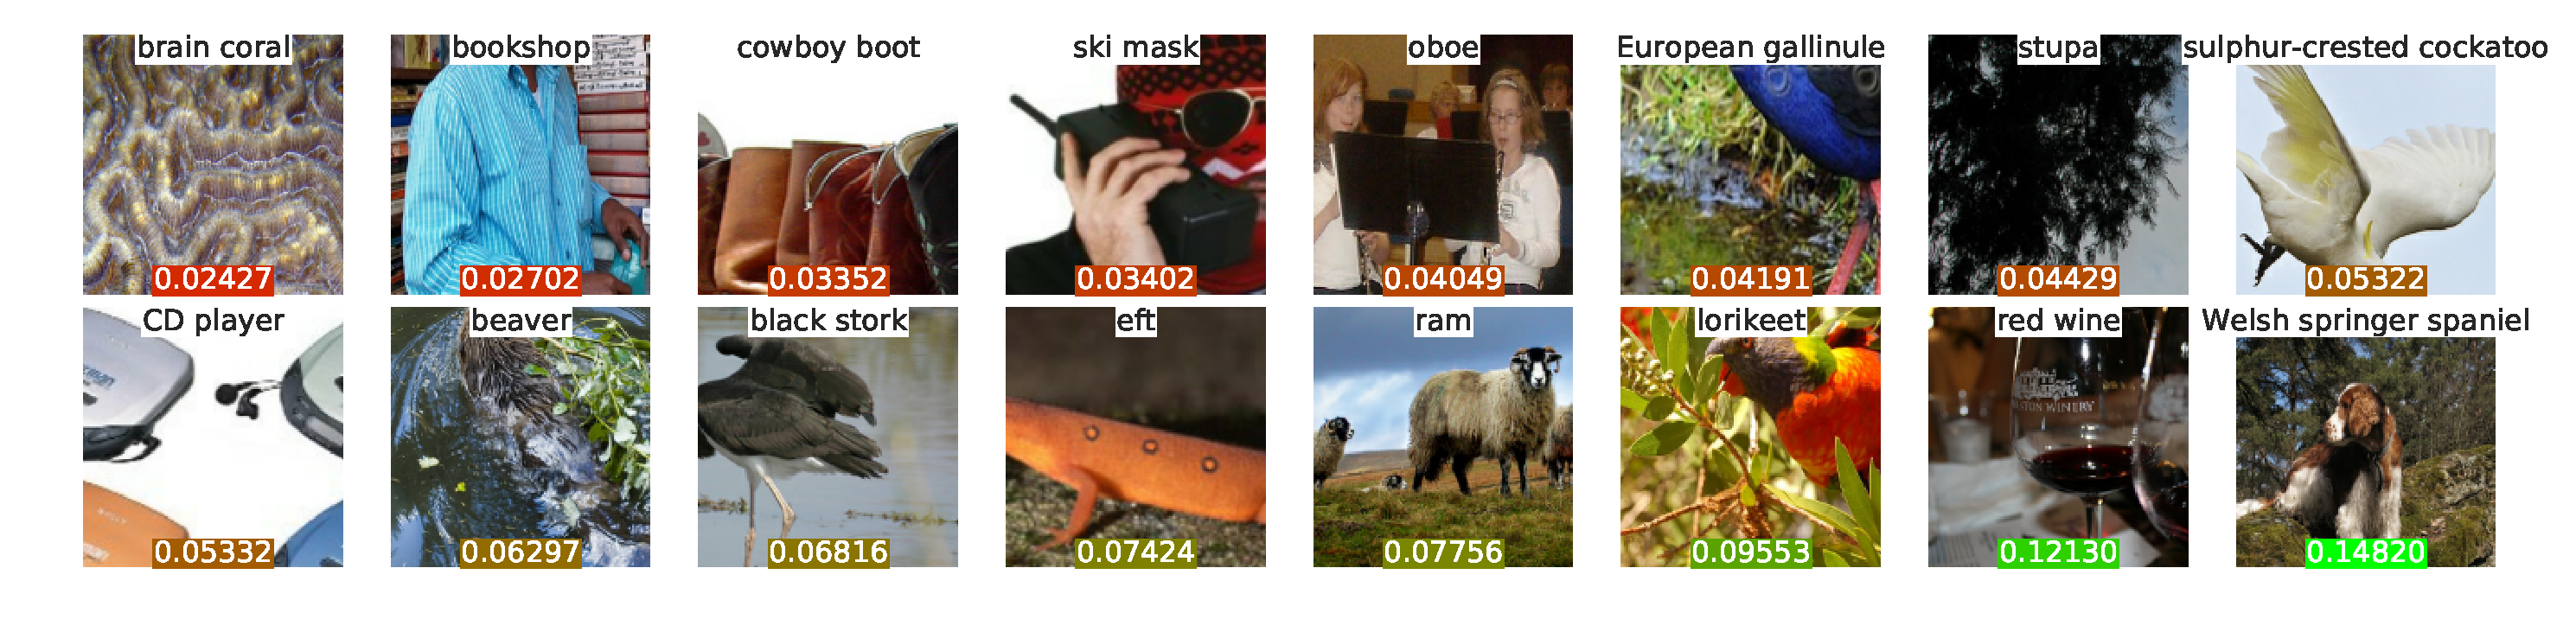
\includegraphics[width=\textwidth]{figs/imagenet_dds.eps}
  \caption{\label{fig:dds_score} Example images from the ImageNet and their weights assigned by \dds. }
\end{figure}

\subsection{Analysis of Multilingual NMT}
Next, we focus on multilingual NMT, where the choice of data directly corresponds to picking a language, which has an intuitive interpretation. Since \dds adapts the data weights dynamically to the model throughout training, here we analyze how the learned weights change throughout training.
%\begin{center}
%  \includegraphics[width=0.245\columnwidth]{figs/aze_devppl_plot.eps}
%  \includegraphics[width=0.23\columnwidth]{figs/bel_devppl_plot.eps}
%  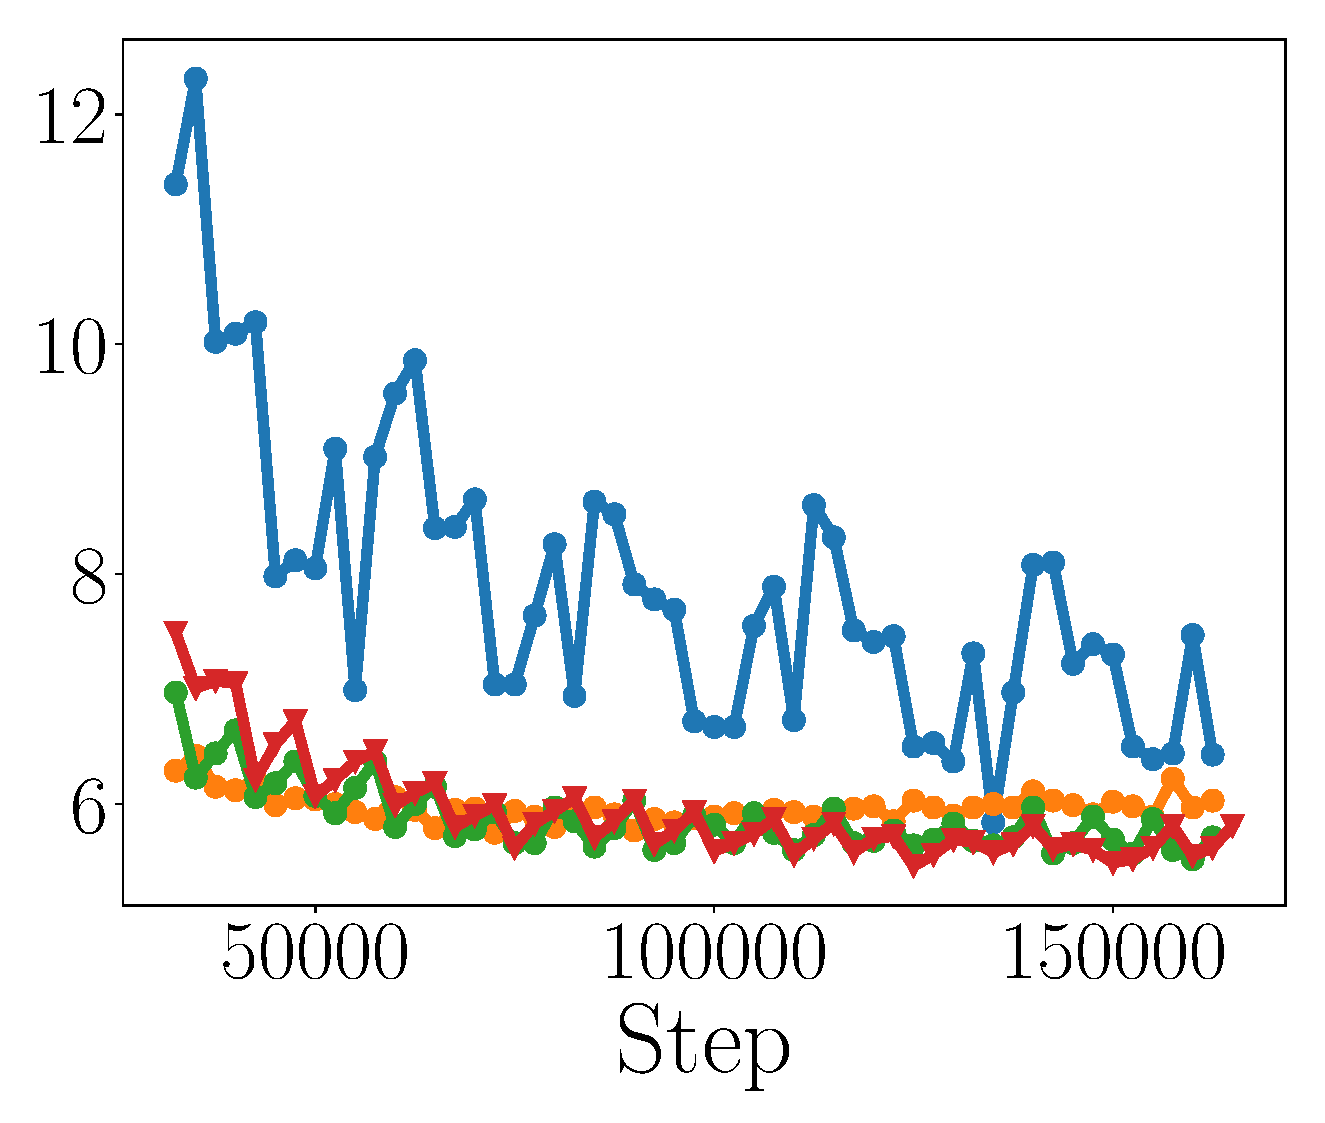
\includegraphics[width=0.23\columnwidth]{figs/glg_devppl_plot.eps}
%  \includegraphics[width=0.23\columnwidth]{figs/slk_devppl_plot.eps}
%  \captionof{figure}{\label{fig:nmt_converge}Development set perplexity vs. training steps. \textit{From left to right}: \texttt{aze}, \texttt{bel}, \texttt{glg}, \texttt{slk}.}
%\end{center}
%\paragraph{Training Curves.} First, we plot the dev set perplexity for three training methods, TCS, DDS, and TCS+DDS over the course of training in Figure \ref{fig:nmt_converge}.%
%\footnote{We did not plot ``Uniform'' here because it takes a far larger number of training steps to converge due to its uniform sampling of eight different languages, and thus is not visible on the same scale.}
%From the results, we can see that while DDS starts out with a higher perplexity than the TCS heuristics (which a-priori calculates the most appropriate language to be using based on surface statistics), it quickly catches up and surpasses TCS on all 4 languages.
%In addition, when initialized with the TCS heuristic, DDS starts at a relatively good perplexity and converges even faster.

\begin{center}
  \includegraphics[width=0.22\columnwidth]{figs/aze_hs_probs_plot.eps}
  \includegraphics[width=0.22\columnwidth]{figs/bel_hs_probs_plot.eps}
  \includegraphics[width=0.22\columnwidth]{figs/glg_hs_probs_plot.eps}
  \includegraphics[width=0.29\columnwidth]{figs/slk_hs_probs_plot.eps}
  \captionof{figure}{\label{fig:nmt_distrib_hs}Language usage for TCS$+$DDS by training step. \textit{From left to right}: \texttt{aze}, \texttt{bel}, \texttt{glg}, \texttt{slk}.}
\end{center}

%\paragraph{Learned Language Distributions.}
We plot the probability distribution of the four HRLs (because they have more data and thus larger impact on training) over the course of training.  Figure \ref{fig:nmt_distrib_hs} shows the change of language distribution for TCS+DDS. Since TCS selects the language with the largest vocabulary overlap with the LRL, the distribution is initialized to focus on the most related HRL. For all four LRLs, the percentage of their most related HRL starts to decrease as training continues. For \texttt{aze}, DDS quickly comes back to using its most related HRL. However, for \texttt{bel}, DDS continues the trend of using all four languages. This shows that DDS is able to maximize the benefits of the multilingual data by having a more balanced usage of all languages. 
%For gig and slk, DDS learns to mainly use both por and ces, their corresponding HRL.

\vspace{-0.2cm}
\begin{center}
  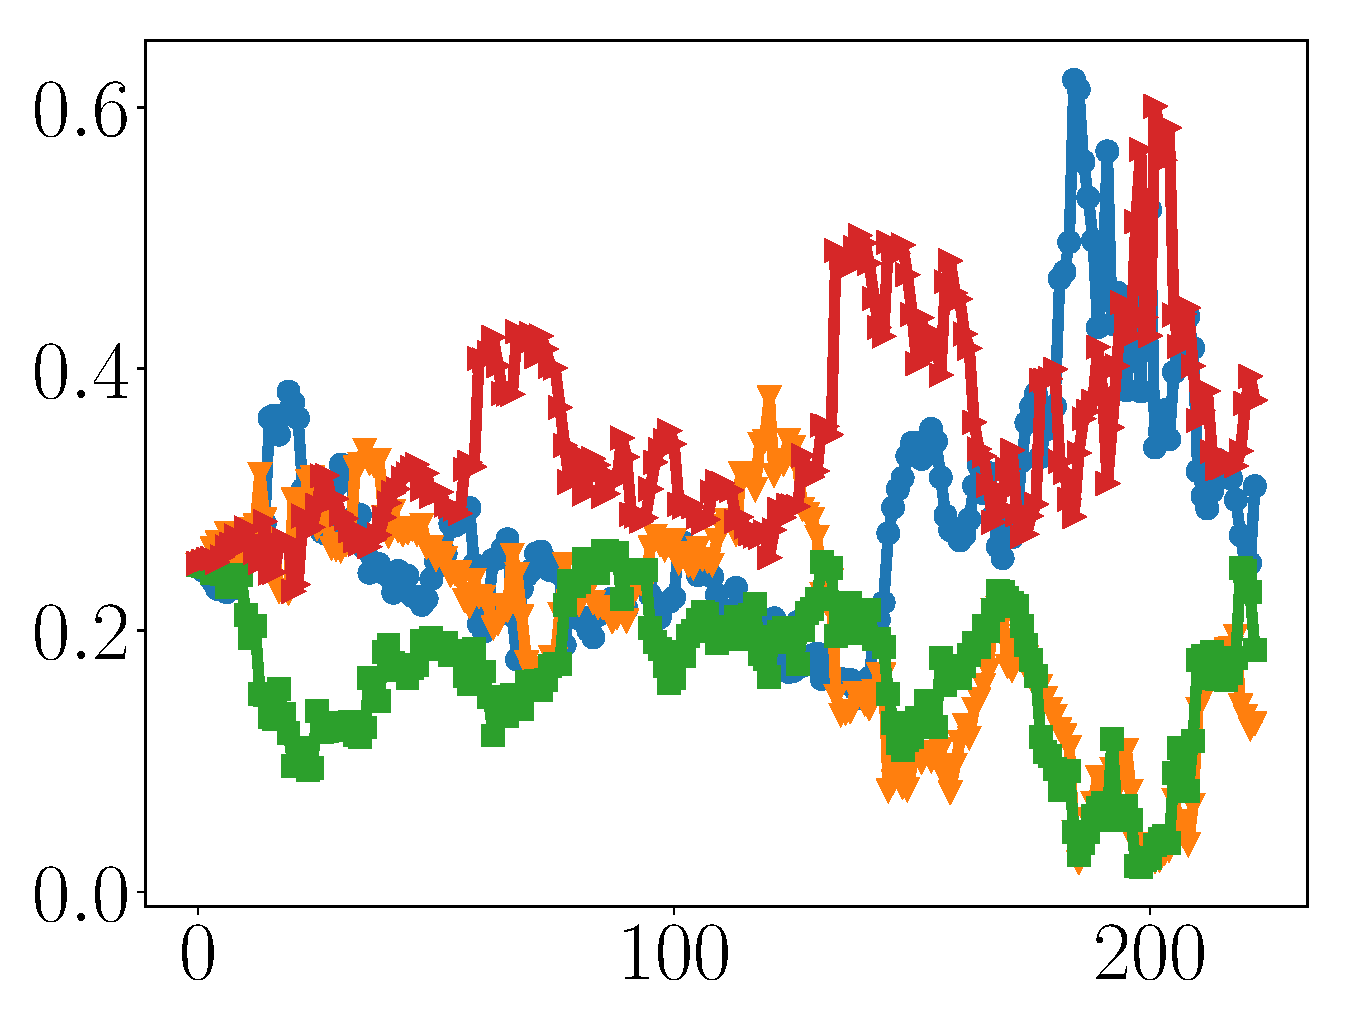
\includegraphics[width=0.22\columnwidth]{figs/aze_uni_probs_plot.eps}
  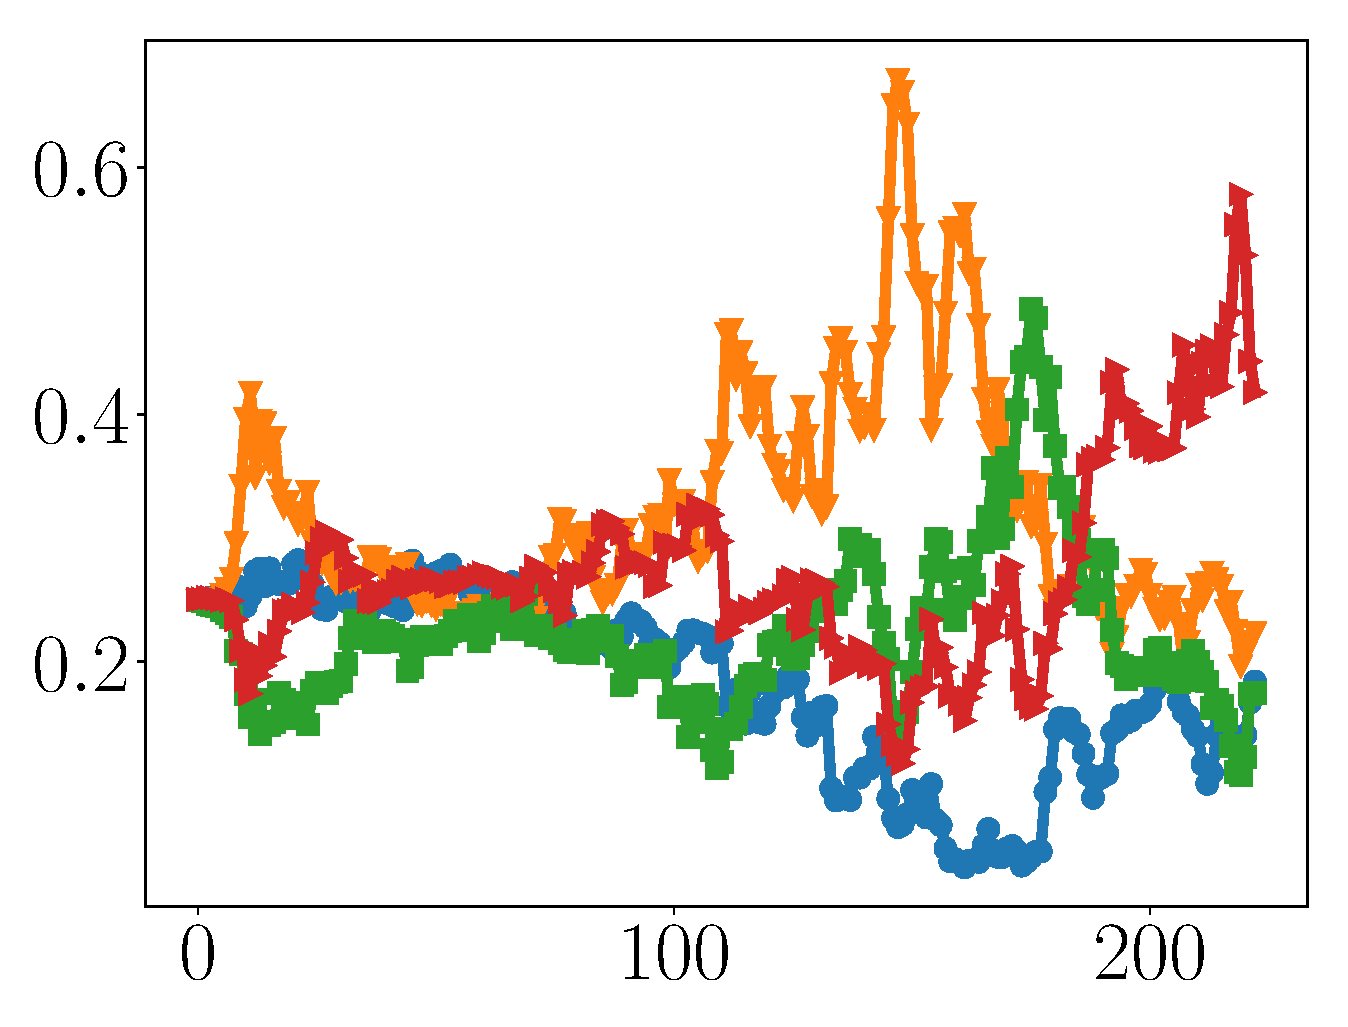
\includegraphics[width=0.22\columnwidth]{figs/bel_uni_probs_plot.eps}
  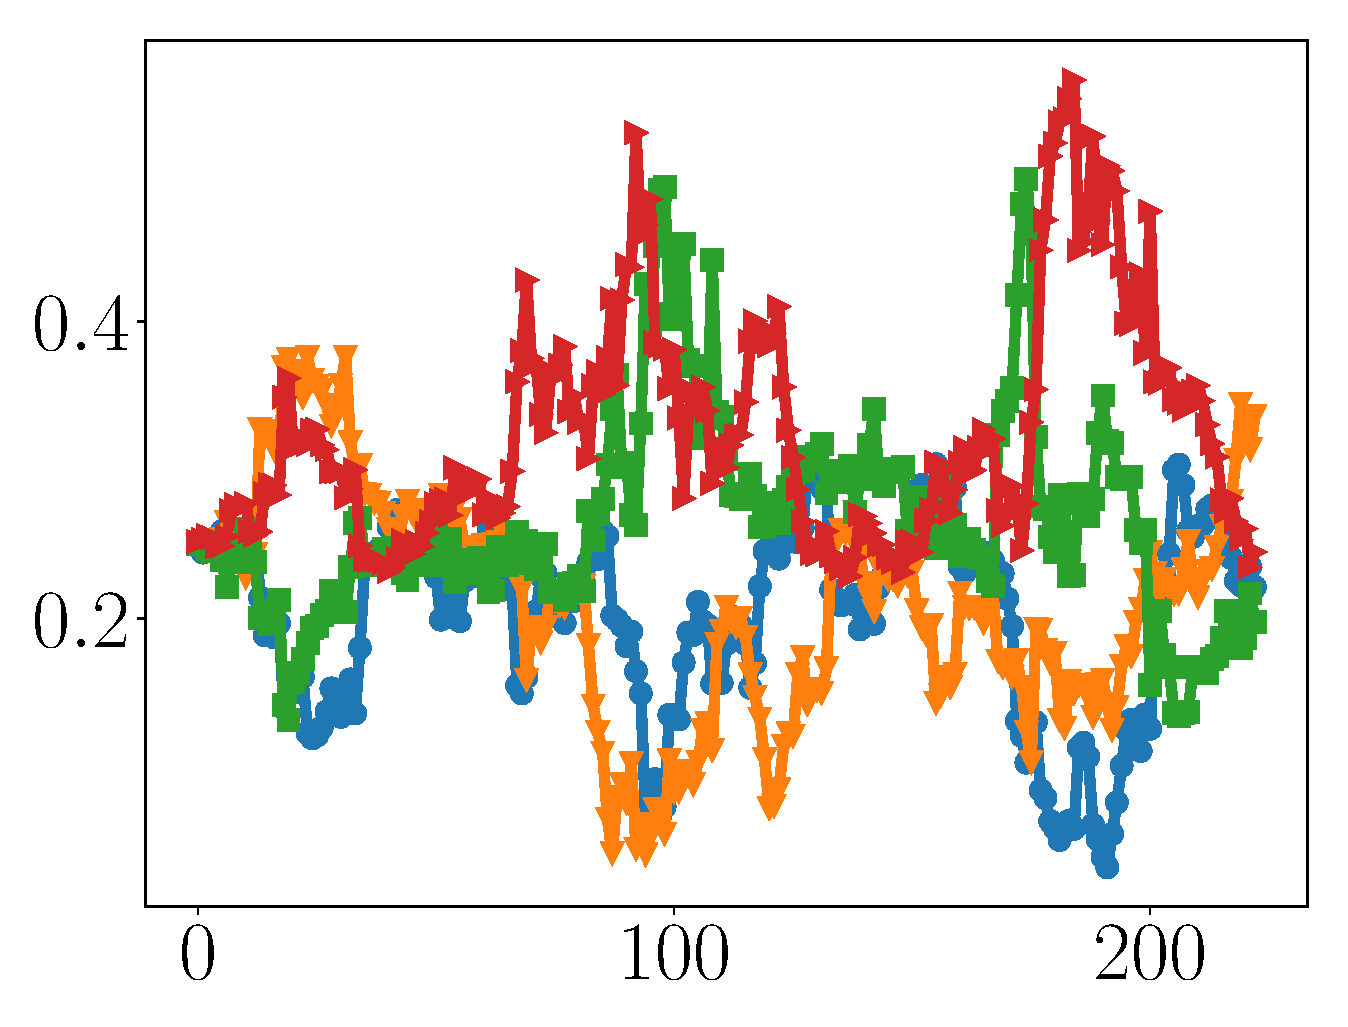
\includegraphics[width=0.22\columnwidth]{figs/glg_uni_probs_plot.eps}
  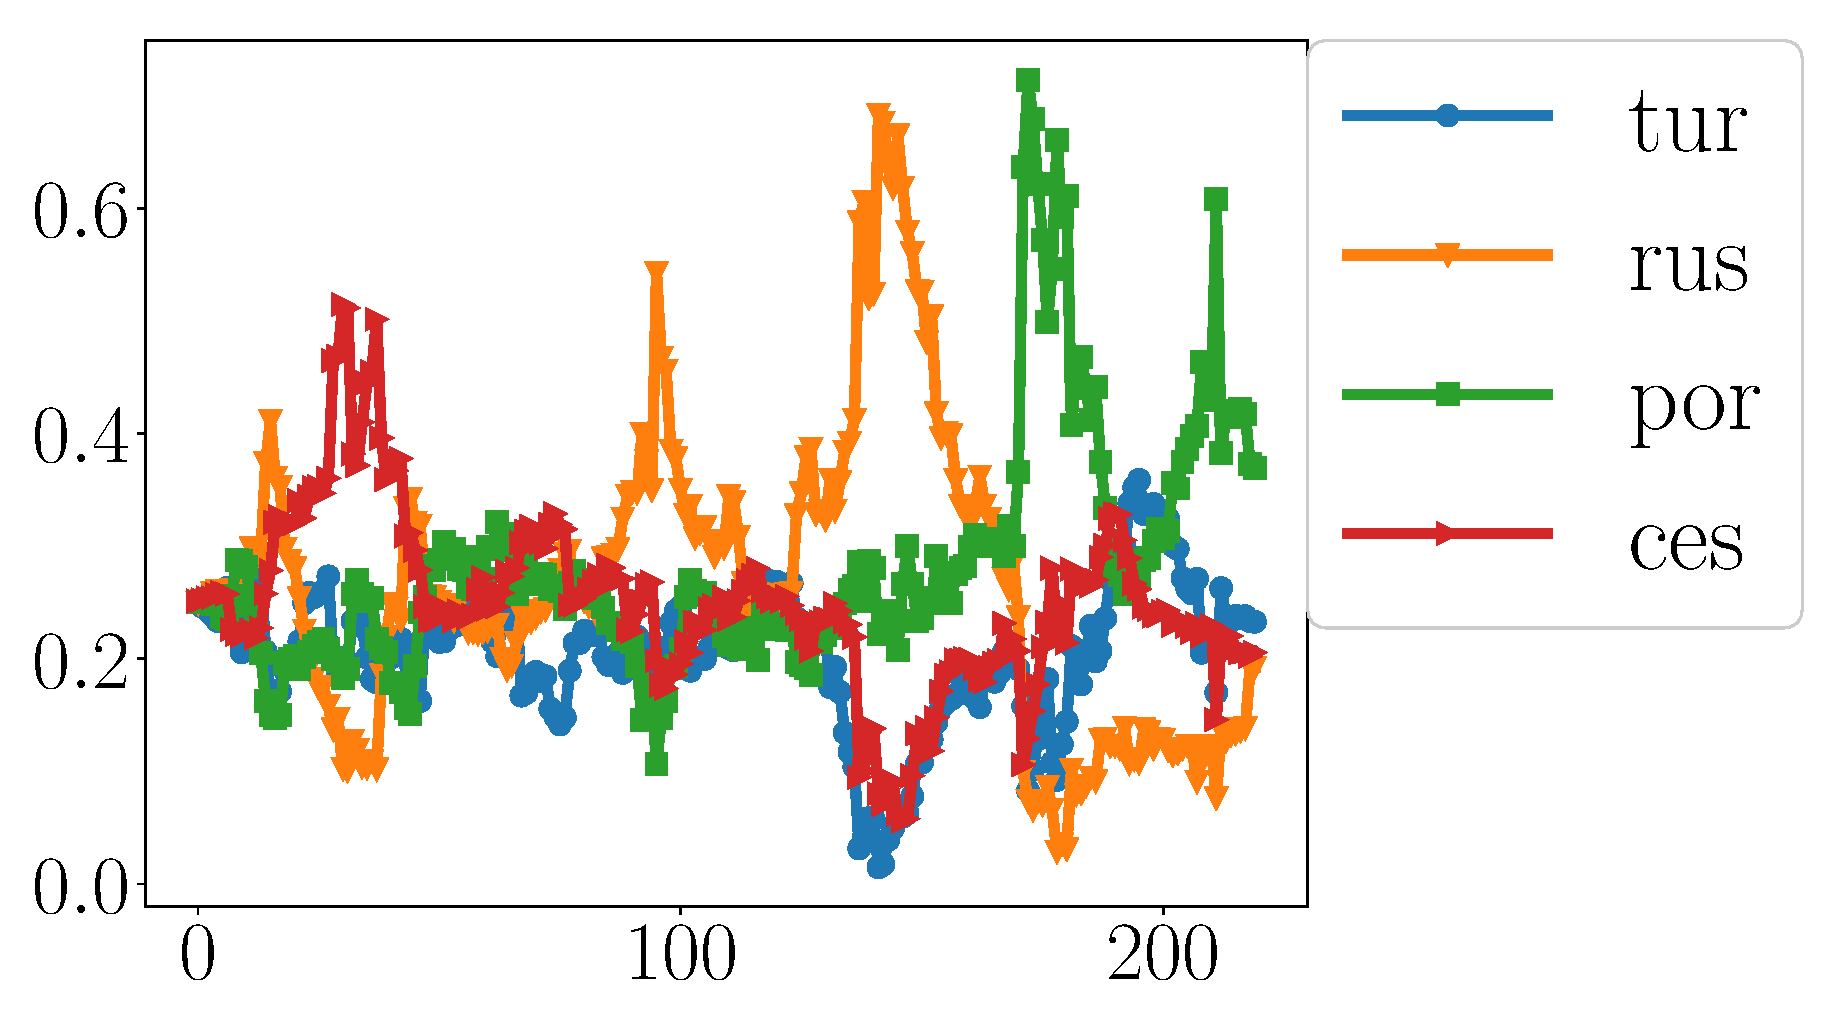
\includegraphics[width=0.29\columnwidth]{figs/slk_uni_probs_plot.eps}
  \captionof{figure}{\label{fig:nmt_distrib_uni}Language usage for DDS by training step. \textit{From left to right}: \texttt{aze}, \texttt{bel}, \texttt{glg}, \texttt{slk}.}
\end{center}
\vspace{-0.2cm}

In Figure \ref{fig:nmt_distrib_uni}, we show a more interesting trend of DDS without heuristic initialization.
For both \texttt{aze} and \texttt{bel}, our method learns to focus on their most related HRL after a certain number of training updates.
Interestingly, for \texttt{bel}, DDS learns to focus on both \texttt{rus}, its most related HRL, and another language \texttt{ces}. Similarly for \texttt{slk}, DDS also learns to focus on \texttt{ces}, its most related HRL, and \texttt{rus}, although there is little vocabulary overlap between \texttt{slk} and \texttt{rus}.
Also notably, the ratios significantly change over the course of training, indicating that different types of data may be more useful during different stages of learning the model.
Notably, DDS shows significant improvements over uniform sampling and other heuristics, demonstrating that it is able to discover when it should use other data, even if the patterns are not immediately intuitive.
%Similar to the trend in Figure \ref{fig:nmt_distrib_hs}, glg tends to use both por, its most related HRL, and ces. 

\section{\label{sec:related_work}Related Works}
%\gn{These are mostly based on stuff for NMT, a broader survey is necessary to increase more general ML methods. I've also only added a small subset of the papers on MT. Please follow the backward and forward references (forward references can be found by clicking the ``cited by'' link in Google Scholar).}

For both NMT and image classification, several prior work has focused on data selection for domain adaptation~\citep{moore2010intelligent,axelrod2011domain,domain_adapt_transfer,jiang-zhai-2007-instance,foster-etal-2010-discriminative,wang-etal-2017-instance}, generally using heuristics to measure domain similarity. \cite{domain_adapt_transfer} propose to estimate the importance weight of the classification labels in the pretraining dataset to mitigate the domain differences, while DDS is a more general data selection framework that works for both classification and other usage cases. Besides domain adaptation, it is also found that selecting good examples from the training data can improve NMT~\citep{vyas-etal-2018-identifying,pham-etal-2018-fixing}.  

The formulation of DDS involves bilevel optimization~\citep{bilevel_optim,hier_optim}, which is utilized in several prior work in areas other than data selection~\citep{darts,hyper_grad,finn2017model}. Notably, \cite{darts} proposes a nested optimization to link training and dev set, similar to the general philosophy behind DDS. \cite{darts} utilizes this formulation for efficient neural architecture search, while DDS is designed for efficient data usage.

More generally, our method is also related to the general machine learning problem of teaching. Firstly, hardness-based teaching in curriculum learning estimate the curriculum based on an heuristic understading of the hardness of data~\citep{cl_bengio,automate_cl_GravesBMMK17,SpitkovskyAJ10,zhang2016boosting,zhang2018empirical,platanios19naacl,baysian_curriculum}. These methods, though effective, are harder to generalize because they often require task-specific features. On the other hand, self-paced learning~\citep{spl_visual_category,spl_kumar,spl_visual_category} defines the hardness of the data based on the loss from the main model. This method requires less heuristic estimates, but is still based on the assumption that easy examples should be learned first. Secondly, the recently proposed learning to teach~\citep{learn_to_teach} is probably closer to our setting, where they train a teacher model so that it can ``teach'' the main model better. However, their method requires featurizing the data and student models so that the teacher model could be trained with reinforcement learning. In comparison, our method focuses on data selection, and provides a much simpler framework without feature engineering. 

%Lastly, our method is related to the work on investigating the effect of label noise on deep image recognition models \cite{rolnick2017deep,overfit_random_examples} or machine translation \cite{khayrallah-koehn-2018-impact}, while \citet{koh2017understanding} shows the feasibility of training set poisoning attacks.


%Instance weighting: \cite{jiang-zhai-2007-instance,foster-etal-2010-discriminative,wang-etal-2017-instance}. In particular, \cite{wang-etal-2017-instance} seems like a good paper to compare against because it's recent and based on neural MT.

%Curriculum learning: \cite{zhang2016boosting,zhang2018empirical,platanios19naacl}.

%Data selection: \cite{moore2010intelligent,axelrod2011domain}.

%Removing bad training examples improves MT: \cite{vyas-etal-2018-identifying,pham-etal-2018-fixing}

%Dataset poisoning (for neural models): \cite{koh2017understanding}



%Meta-learning. Formulation of using the gradient update equation is similar to MAML \cite{finn2017model}.
\section{\label{sec:conclusion}Conclusion}
We present Differentiable Data Selection, an automatic data selection framework for optimizing data usage of deep learning models. Our method does not require domain knowledge for heuristic design, and instead directly optimizes the training data distribution along with the main model. We formulate two algorithms under the DDS framework for both multilingual NMT and image classification, which lead to consistent improvement over strong baselines. 



\bibliography{main}
\bibliographystyle{plainnat}

\newpage
\appendix
\section{\label{app} Appendix}

\subsection{\label{app:grad_of_optimizers}Deriving $\nabla_\psi g$ for Different Optimizers}
%\gn{It seems reasonable to have this as a top-level section, so I changed it accordingly this has started to get into details that are probably better to separate from the overall high-level idea of DDS.}

Here we first derive $\nabla_\psi g$ for the general stochastic gradient descent~(SGD) update, then provide examples for two other common optimization algorithms, namely Momentum~\citep{nesterov} and Adam~\citep{adam}.
%\gn{It's not clear to me why you skip standard SGD without momentum? It seems like it'd make the most sense to start there, even if that's not what you finally use in experiments. If you use it in experiments then you definitely need to discuss it. Then when you explain momentum you could just point out the differences.}

\paragraph{SGD Updates.} The SGD update rule for $\theta$ is as follows
\begin{equation}
  \label{eqn:sgd_update}
   \small
  \begin{aligned}
    \theta_t &\leftarrow \theta_{t-1} - \eta_t \nabla_\theta J(\theta_{t-1}, \psi)
  \end{aligned}
\end{equation}
where $\eta_t$ is the learning rate. Matching the updates in Eqn~\ref{eqn:sgd_update} with the generic framework in Eqn~\ref{eqn:theta_update_rule}, we can see that $g$ in Eqn~\ref{eqn:theta_update_rule} has the form: %\gn{$J(\theta_{t-1})$ should be $J(\theta_{t-1}, \psi)$? There seem to be a few of these inconsistencies below as well, so please check. Also, which time step of $\theta$ does the gradient depend on?}
\begin{equation}
  \label{eqn:momentum_update_g}
   \small
  \begin{aligned}
    g\big(\nabla_\theta J(\theta_{t-1}, \psi)\big) = \eta_t \nabla_\theta J(\theta_{t-1}, \psi)
  \end{aligned}
\end{equation}
This reveals a linear dependency of $g$ on $\nabla_\theta J(\theta_{t-1, \psi})$, allowing the exact differentiation of $g$ with respect to $\psi$. From Eqn~\ref{eqn:psi_update_rule}, we have
\begin{equation}
  \label{eqn:momentum_update_for_psi}
   \small
  \begin{aligned}
    &\nabla J(\theta_t, \mathcal{D}_\text{dev})^\top \cdot \nabla_\psi g\big( \nabla_\theta J(\theta_{t-1}, \psi) \big) \\
    &= \eta_t \cdot \nabla_\psi \mathbb{E}_{x, y \sim p(X, Y; \psi)} \left[J(\theta_t, \mathcal{D}_\text{dev})^\top \cdot \nabla_\theta \ell(x, y; \theta_{t-1} )\right] \\
    &= \eta_t \mathbb{E}_{x, y \sim p(X, Y; \psi)} \left[\left( J(\theta_t, \mathcal{D}_\text{dev})^\top \cdot \nabla_\theta \ell(x, y; \theta_{t-1} ) \right) \cdot \nabla_\psi \log{p(x, y; \psi)} \right]
  \end{aligned}
\end{equation}
%\gn{This last paragraph was too dense for me to follow: could you please try to explain a little more?}
Here, the last equation follows from the log-derivative trick in the REINFORCE algorithm~\citep{reinforce}. 
%and can be implemented by Monte Carlo approximation.
%\gn{again, a little more detail here would be useful}. 
%Note we do not do reinforcement learning in this paper. Instead \gn{this ``instead'' was also not clear to me.}, we simply utilize the same log-derivative trick to compute $\nabla_\psi J(\theta_t, \mathcal{D}_\text{dev})$. 

\paragraph{Momentum Updates.} The momentum update rule for $\theta$ is as follows
\begin{equation}
  \label{eqn:momentum_update}
   \small
  \begin{aligned}
    m_t &\leftarrow \mu_t m_{t-1} + \eta_t \nabla_\theta J(\theta_{t-1}, \psi) \\
    \theta_t &\leftarrow \theta_{t-1} - m_t,
  \end{aligned}
\end{equation}
where $\mu_t$ is the momentum coefficient and $\eta_t$ is the learning rate. This means that $g$ has the form:
\begin{equation}
  \label{eqn:momentum_update_g}
   \small
  \begin{aligned}
    g(x) &= \mu m_{t-1} + \eta_t x \\
    g'(x) &= \eta_t
  \end{aligned}
\end{equation}
Therefore, the computation of the gradient $\nabla_{\psi}$ for the Momentum update is exactly the same with the standard SGD update rule in Eqn \ref{eqn:momentum_update_for_psi}.


\paragraph{Adam Updates.} We use a slightly modified update rule based on Adam~\citep{adam}:
\begin{equation}
  \label{eqn:adam_update}
   \small
  \begin{aligned}
    &g_t \leftarrow \nabla_\theta J(\theta_{t-1}, \psi) \\
    &v_t \leftarrow \beta_2 v_{t-1} + (1 - \beta_2) g_t^2 \\
    &\hat{v}_t \leftarrow v_t / (1 - \beta_2^t) \\
    &\theta_t \leftarrow \theta_{t-1} - \eta_t \cdot g_t / \sqrt{\hat{v}_t + \epsilon}
  \end{aligned}
\end{equation}
where $\beta_2$ and $\eta_t$ are hyper-parameters. This means that $g$ is a component-wise operation of the form:
\begin{equation}
  \label{eqn:adam_update_g}
   \small
  \begin{aligned}
    g(x) &= \frac{\eta_t \sqrt{1 - \beta_2^t} \cdot x}{\sqrt{\beta_2 v_{t-1} + (1 - \beta_2) x^2 + \epsilon}} \\
    g'(x) &= \frac{\eta_t \sqrt{1 - \beta_2^t} (\beta_2 v_{t-1} + \epsilon)}{\big( \beta_2 v_{t-1} + (1 - \beta_2) x^2 + \epsilon \big)^{3/2}} \approx \eta_t \sqrt{\frac{1 - \beta_2^t}{\beta_2 v_{t-1}}},  
  \end{aligned}
\end{equation}
%\paul{So all of this is under the assumption that $v_{t-1}$ is independent on $\psi$ right? maybe bring it up?}
the last equation holds because we assume $v_{t-1}$ is independent of $\psi$. Here the approximation makes sense because we empirically observe that the individual values of the gradient vector $\nabla_\theta J(\theta_{t-1}, \psi)$,~\ie~$g_t$, are close to $0$. Furthermore, for Adam, we usually use $\beta_2 = 0.999$. Thus, the value $(1 - \beta_2) x^2$ in the denominator of Eqn~\ref{eqn:adam_update_g} is negligible. With this approximation, the computation of the gradient $\nabla_\psi$ is almost the same with that for SGD in Eqn~\ref{eqn:momentum_update_for_psi}, with one extra component-wise scaling by the term in Eqn~\ref{eqn:adam_update_g}.

\subsection{\label{app:nmt_hparam} Hyperparameters for multilingual NMT}
In this section, we give a detailed description of the hyperparameters used for the multilingual NMT experiments.
\begin{itemize}
    \item We use a 1 layer LSTM with hidden size of 512 for both the encoder and decoder, and set the word embedding to size 128.
    \item The dropout rate is set to 0.3.
    \item For the NMT model, we use Adam optimizer with learning rate of 0.001. For the distribution parameter $\psi$, we use Adam optimizer with learning rate of 0.0001.
    \item We train all models for 20 epochs without any learning rate decay.
\end{itemize}

\subsection{\label{app:nmt_data} Dataset statistics for Multilingual NMT}
\begin{table}[H]
%\begin{wraptable}{r}{4.3cm}
  \centering
   %\resizebox{0.3\textwidth}{!}{
  \begin{tabular}{c|ccc|cc}
  \toprule
  \textbf{LRL} & \textbf{Train} & \textbf{Dev} & \textbf{Test} & \textbf{HRL} & \textbf{Train} \\
  \midrule
  aze & 5.94k &  671 &  903 & tur & 182k \\
  bel & 4.51k &  248 &  664 & rus & 208k \\
  glg & 10.0k &  682 & 1007 & por & 185k \\
  slk & 61.5k & 2271 & 2445 & ces & 103k \\
  \bottomrule
  \end{tabular}
  %}
  \vspace{0.2cm}
  \caption{\label{tab:nmt_data}Statistics of the multilingual NMT datasets.}
% \end{wraptable}
\end{table} 

\subsection{\label{app:image_hparam} Hyperparameters for image classification}
In this section, we provide some additional details for the image classification task:
\begin{itemize}
  \item We use the cosine learning rate decay schedule~\citep{cosine_lr}, starting at $0.1$ for CIFAR-10 and $3.2$ for ImageNet, both with $2000$ warmup steps. 
  \item We maintain a moving average of all model parameters with the rate of $0.999$. Following~\citet{imagenet_generalize_better}, we treat the moving statistics of batch normalization~\citep{batch_norm} as \textit{untrained parameters} and also add them to the moving averages. 
\end{itemize}

%\subsection{\label{app:image_detail} Training details for image classification}
%Our experiments were conducted on second-generation Tensor Processing Units (TPUv2). There were several important implementation details related to improving training efficiency with DDS for ImageNet models (these were not needed for the smaller CIFAR-10 training set). First, each batch of $4096$ training instances for ImageNet is processed in parallel on $32$ TPU cores, each working on $128$ images. When we compute $p(\hat{x}, \hat{y}; \psi)$ (in~Section \ref{sec:image_method}), the softmax function is computed \textit{locally on each core} to reduce the synchronization overhead. Second, since we do not need the parameters $\psi$ of the DDS model, we ignore all batch normalization moving average updates when we pass images through $p(\hat{x}, \hat{y}; \psi)$. We also only batch-normalize the DDS model locally on each TPU core. Controlled profiling measures show that the aforementioned details speed up the training process by almost $2.5 \times$. Third, following~\citet{neural_combi} and~\citet{enas}, for ImageNet, we apply a $\tanh$ activation to the logits prior to the softmax to compute $p(\hat{x}, \hat{y}; \psi)$, which softens the softmax distribution and prevents the $p(\hat{x}, \hat{y}; \psi)$ from collapsing into always choosing a particular example.

\subsection{Training Time}
For NMT, the baseline TCS takes 10 hours, and DDS takes about 24 hours to finish. Our NMT code is not optimized and can potentially be made much more efficient. 
For CIFAR-10, DDS take about $9$ hours, while experiments without DDS takes $5.5$ hours, and for ImageNet, these take $4$ hours and $6$ hours approximately. 



\end{document}